\section{Experiment 2: Mathematical analysis of the network with 1-D images}
\label{section:1D}

\subsection{Introduction}

The purpose of this experiment was to analyse a smaller network and provide a definitive way to verify the performance of the simulation. Furthermore, the weights were not learned as in the previous experiment, but rather determined analytically. This was done to experimentally prove the relation given by \citet{nessler} that the weights stochastically converge toward the conditional probability that a presynaptic neuron fired shortly before the postsynaptic neuron.
First the network was scaled down to be one-dimensional with 18 input neurons, four prior neurons and four output neurons, making it easier to analyse. The weights were determined by utilizing the logarithmic connection between them and the corresponding conditional probabilities, as given by Equation \ref{eqn:weightProbLink}. The conditional probabilities of the input and output neurons of the network  were calculated and then used to determine the posterior probability of the network. After the simulation of the network the distribution of the output spikes was used to calculate the posterior probability. The posterior probabilities of both the mathematical analysis and the simulation were compared. By varying three network hyperparameters it was tuned to approximate the analytical solution as closely as possible.

\subsection{Methods}

\paragraph{Input data}
The input image consisted of nine pixels in a horizontal line. Within those nine pixels, going from position 0 to 8, four output classes could be represented. Each output class had of three pixels next to each other. This resulted in each output class overlapping its neighbour classes by one pixel. Thus the centers of the output classes were at position 1, 3, 5 and 7.
 
\paragraph{Network architecture}
Compared to the architecture of the previous experiment only the amount of neurons was changed. As there have to be 2 input neurons for each pixel, one neuron being active if the pixel is white and one if the pixel is black, the network had 18 input neurons. Furthermore four prior neurons were implemented, of which only one is being active for one of the output classes at a time. Lastly the network had four output neurons.

\paragraph{Mathematical Analysis}
The posterior probability of the network was calculated by using Equation \ref{eqn:pYvorausgesetztXUndZ}.
$P(X=x|Y=k)$ and $P(Y=k|Z=j)$ were derived corresponding to the paradigm of the experiment.
 The calculation of $P(X=x|Y=k)$ was split into two parts. First the contribution of the active input neurons was calculated by determining the matrix $P^{X|Y}$. This matrix is of size 4 x 9 and contains the conditional probabilities of each input neuron $y_k$ being active, given that an output neuron $x_i$ is active. These probabilities were calculated by determining which input neurons are active depending on the output class and which input neurons are inactive, as dictated by the network architecture. Furthermore, the noise that was applied to the input neurons had to be taken into account. For input neurons belonging to the output class the conditional probability was determined as 1 and lowered by the noise level, while for the input neurons outside of the 3-wide pixel block belonging to the output class it was determined as 0 and raised by the noise level. According to this $P^{X|Y}$ is given by
\begin{equation}
\label{eqn:PXvorausgesetztYIf}
P_{k,i}^{X|Y} = \begin{dcases*} 1 - $noise level$ & if $x_i$ is in the active area of $y_k$, \\
0 + $noise level$ & \text{if $x_i$ is not in the active area of $ y_k $ } \end{dcases*}.\end{equation}
  After calculating all entries of $P^{X|Y}$ its rows were multiplied with the input image vector
\begin{equation}
\label{eqn:p1XvorausgesetztYMalX}
P_1(X = x|Y = k) = P^{X|Y}_{k,*} \cdot x
\end{equation}
resulting in a conditional probability for each output class depending on the input vector. The input vector was given with entries of 1 for active pixels and with entries of 0 for inactive pixels.
Next to include the contribution of the input neurons that are spiking when a pixel is inactive the conditional probability of the input neurons that are active for the entries where $x_i = 0$ had to be calculated. To achieve this complementary conditional probability at first $P^{X|Y}$ was subtracted from one. To include the correct conditional probabilities for the complementary case the input image vector x was then also subtracted from one. $1 - P^{X|Y}$ and $1 - x$ were multiplied to yield
\begin{equation}
\label{eqn:p2minusXvorausgesetztYMalX}
P_2(X = x|Y = k) = (1 - P^{X|Y}_{k,*}) \cdot (1 - x).
\end{equation}
The results of both calculations were then multiplied element-wise to yield
\begin{equation}
\label{eqn:pXvorausgesetztY}
P(X = x|Y = k) = P_1(X = x|Y = k) \odot P_2(X = x|Y = k).
\end{equation}
$P(Y=k|Z=j)$ was determined by first calculating the matrix $P^{Y|Z}$. It has a dimension of 4 x 4 and contains the conditional probabilities for the output neuron $y_k$, given the prior neuron $z_j$ being active. For each output class there exists one corresponding prior neuron. As there can never be more than one active prior neuron at a time $P^{Y|Z}$ is given by
\begin{equation}
\label{eqn:PYvorausgesetztZIf}
P_{k,j}^{Y|Z} = \begin{dcases*} 1 - $noise level$ & if $i = j$, \\
0 +  \frac{1}{3}  $noise level$ & \text{if $i \neq j$. } \end{dcases*}\end{equation} 
$P(Y=k|Z=j)$ was then obtained by
\begin{equation}
\label{eqn:pYvorausgesetztZ}
P(Y=k|Z=j) = P^{Y|Z} \cdot z
\end{equation}
where z is given by a 4 x 1 one-hot encoded vector of the prior.

\paragraph{Simulation}
The input weights for the simulation were calculated as two separate sets. First weights $w^{I1}$ for the input neurons that are active for active input pixels were determined by 
\begin{equation}
\label{eqn:1DWeights}
w^{I1} = \ln(P^{X|Y}).
\end{equation}
Second complementary input weights $w^{I2}$ were calculated for  input neurons representing non active input pixels with
\begin{equation}
\label{eqn:1DWeightsComplementary}
w^{I2} = \ln(1 - P^{X|Y}).
\end{equation} 
The prior weights $w^P$ were derived by 
\begin{equation}
\label{eqn:1DWeightsPrior}
w^P = \ln(P^{Y|Z}).
\end{equation}

The network was simulated for six different input images for each hyperparameter set. These six images were hand-picked to include specific edge cases and to allow comparability of the results of different hyperparameter sets. After the image presentation period of each input image the numbers of output spikes of each class were counted and their proportions were calculated to yield the posterior $P_{simulation}(Y = k|X, Z)$. The Kullback-Leibler divergence was chosen to compare the divergence of the analytic and the simulated posteriors of the network. This metric indicates how much two probability distributions diverge from each other. The goal of the hyperparameter search of the simulation was to minimize the Kullback-Leibler divergence. After showing an output image to the network the Kullback-Leibler divergence was calculated as
\begin{equation}
\begin{split}
\label{eqn:KLDivergence}
D_{KL}(P_{analysis}(Y = k|X, Z)||P_{simulation}(Y = k|X, Z)) = \\ \sum_{k=1}^K P_{analysis}(Y = k|X, Z) \cdot \ln( \frac{P_{analysis}(Y = k|X, Z)}{P_{simulation}(Y = k|X, Z)})
\end{split}
\end{equation}
where K is the number of output neurons and $P_{analysis}(Y = k|X, Z)$ and $P_{simulation}(Y = k|X, Z)$ are the posteriors of the network, later called "analysis output probabilities" and "simulation output probabilities" in plots. The six resulting Kullback-Leibler divergences for each hyperparameter set were  averaged to create a single metric by which the performance of the different hyperparameter sets was compared. The three hyperparameters input firing rate $f_{input}$, prior firing rate $f_{prior}$ and the membrane constant $\tau_{decay}$ were varied to inspect their influence on the result, as well as to approximate the analytical solution as closely as possible. Each input image was presented to the network for 20 seconds to reduce the variance between runs. Furthermore each simulation was repeated 20 times with the same hyperparameter set to obtain the mean and standard deviation of the simulation output probabilities and of the Kullback-Leibler divergence.

\subsection{Results}

\paragraph{Analytic Results}

First the matrix $P^{X|Y}$ was calculated using Equation \ref{eqn:PXvorausgesetztYIf} 
\begin{equation}
\label{eqn:pXvorausgesetztYResult}
P^{X|Y} = \begin{bmatrix}
0.9 & 0.9 & 0.9 & 0.1 & 0.1 & 0.1 & 0.1 & 0.1 & 0.1\\
0.1 & 0.1 & 0.9 & 0.9 & 0.9 & 0.1 & 0.1 & 0.1 & 0.1\\
0.1 & 0.1 & 0.1 & 0.1 & 0.9 & 0.9 & 0.9 & 0.1 & 0.1\\
0.1 & 0.1 & 0.1 & 0.1 & 0.1 & 0.1 & 0.9 & 0.9 & 0.9\\
\end{bmatrix}.
\end{equation}
Next the matrix $P^{Y|Z}$ was calculated using Equation \ref{eqn:PYvorausgesetztZIf} 
\begin{equation}
\label{eqn:pYvorausgesetztZResult}
P^{Y|Z} = \begin{bmatrix}
0.9 & 0.0333 & 0.0333 & 0.0333\\
0.0333 & 0.9 & 0.0333 & 0.0333\\
0.0333 & 0.0333 & 0.9 & 0.0333\\
0.0333 & 0.0333 & 0.0333 & 0.9\\
\end{bmatrix}.
\end{equation} 
For each input image these two matrices were multiplied with the input vector and prior vector as described Equations \ref{eqn:p1XvorausgesetztYMalX}, \ref{eqn:p2minusXvorausgesetztYMalX},  \ref{eqn:pXvorausgesetztY} and \ref{eqn:pYvorausgesetztZ} to yield $P(X = x|Y = i)$ and $P(Y=i|Z=j)$. Using \ref{eqn:pYvorausgesetztXUndZ}  finally yielded the analytical $P(Y = i|X = x, Z = j)$.

\paragraph{Simulation results with prior disabled}
To simplify the hyperparameter fitting process the network was at first simulated with inactive prior neurons. Only after determining the best values for $f_{input}$ and $\tau_{decay}$ the prior neurons were reactivated and $f_{prior}$ was fitted. The values 0.015 seconds and 0.004 seconds for $\tau_{decay}$ were used for the simulation and compared. For each of these values an optimal value for $f_{input}$ was found by looking for the value that yielded the smallest Kullback-Leibler divergence.

\subparagraph{$\tau_{decay} = 0.015 seconds$, $f_{prior} = 0 Hz$}
Values for $f_{input}$ between 10 and 110 Hz in steps of 10 Hz were simulated. After identifying the input firing rate with the smallest Kullback-Leibler divergence the network was simulated again for $f_{input}$ values $\pm$ 10 Hz in steps of 2 Hz. The result of this search can be seen in Figure \ref{fig:1D_KLD_fPrior0_tau15}. This process yielded the best input firing rate of 42 Hz. The results of this hyperparameter combination can be seen in Figure \ref{fig:1D_42_0_15}. In this figure six different input images can be seen in A. The active pixels are shown in black. In B the posterior probabilities of the mathematical analysis are given by the red bars and the posterior probabilities of the simulation are given by the blue bars. Each simulation output probability has its standard deviation marked by a black bar. At the bottom the value of the Kullback-Leibler divergence is given, with its standard deviation. The exact numeric probabilities are given in Table \ref{tab:1D_42_0_15}.

\begin{figure}
\centering
  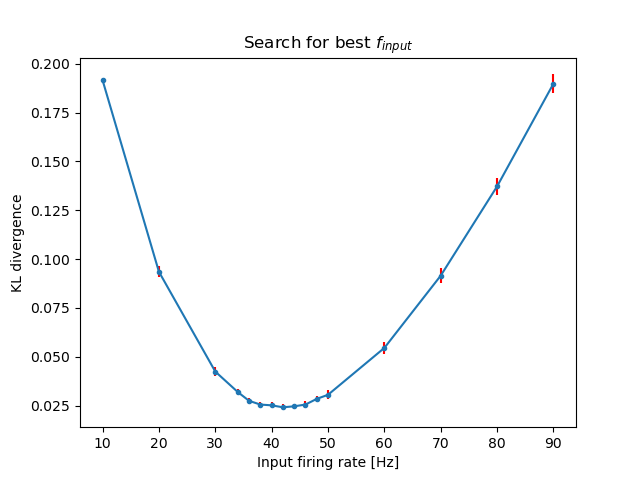
\includegraphics[width=0.75\linewidth]{figures/1D/KLDvsfInput_fPrior0tau15.png}
  \caption{\textbf{KL divergence for different $f_{input}$ values. } Hyperparameters: $f_{prior} = 0 Hz, \tau_{decay} = 15 ms$}
  \label{fig:1D_KLD_fPrior0_tau15}
\end{figure}

\begin{figure}
  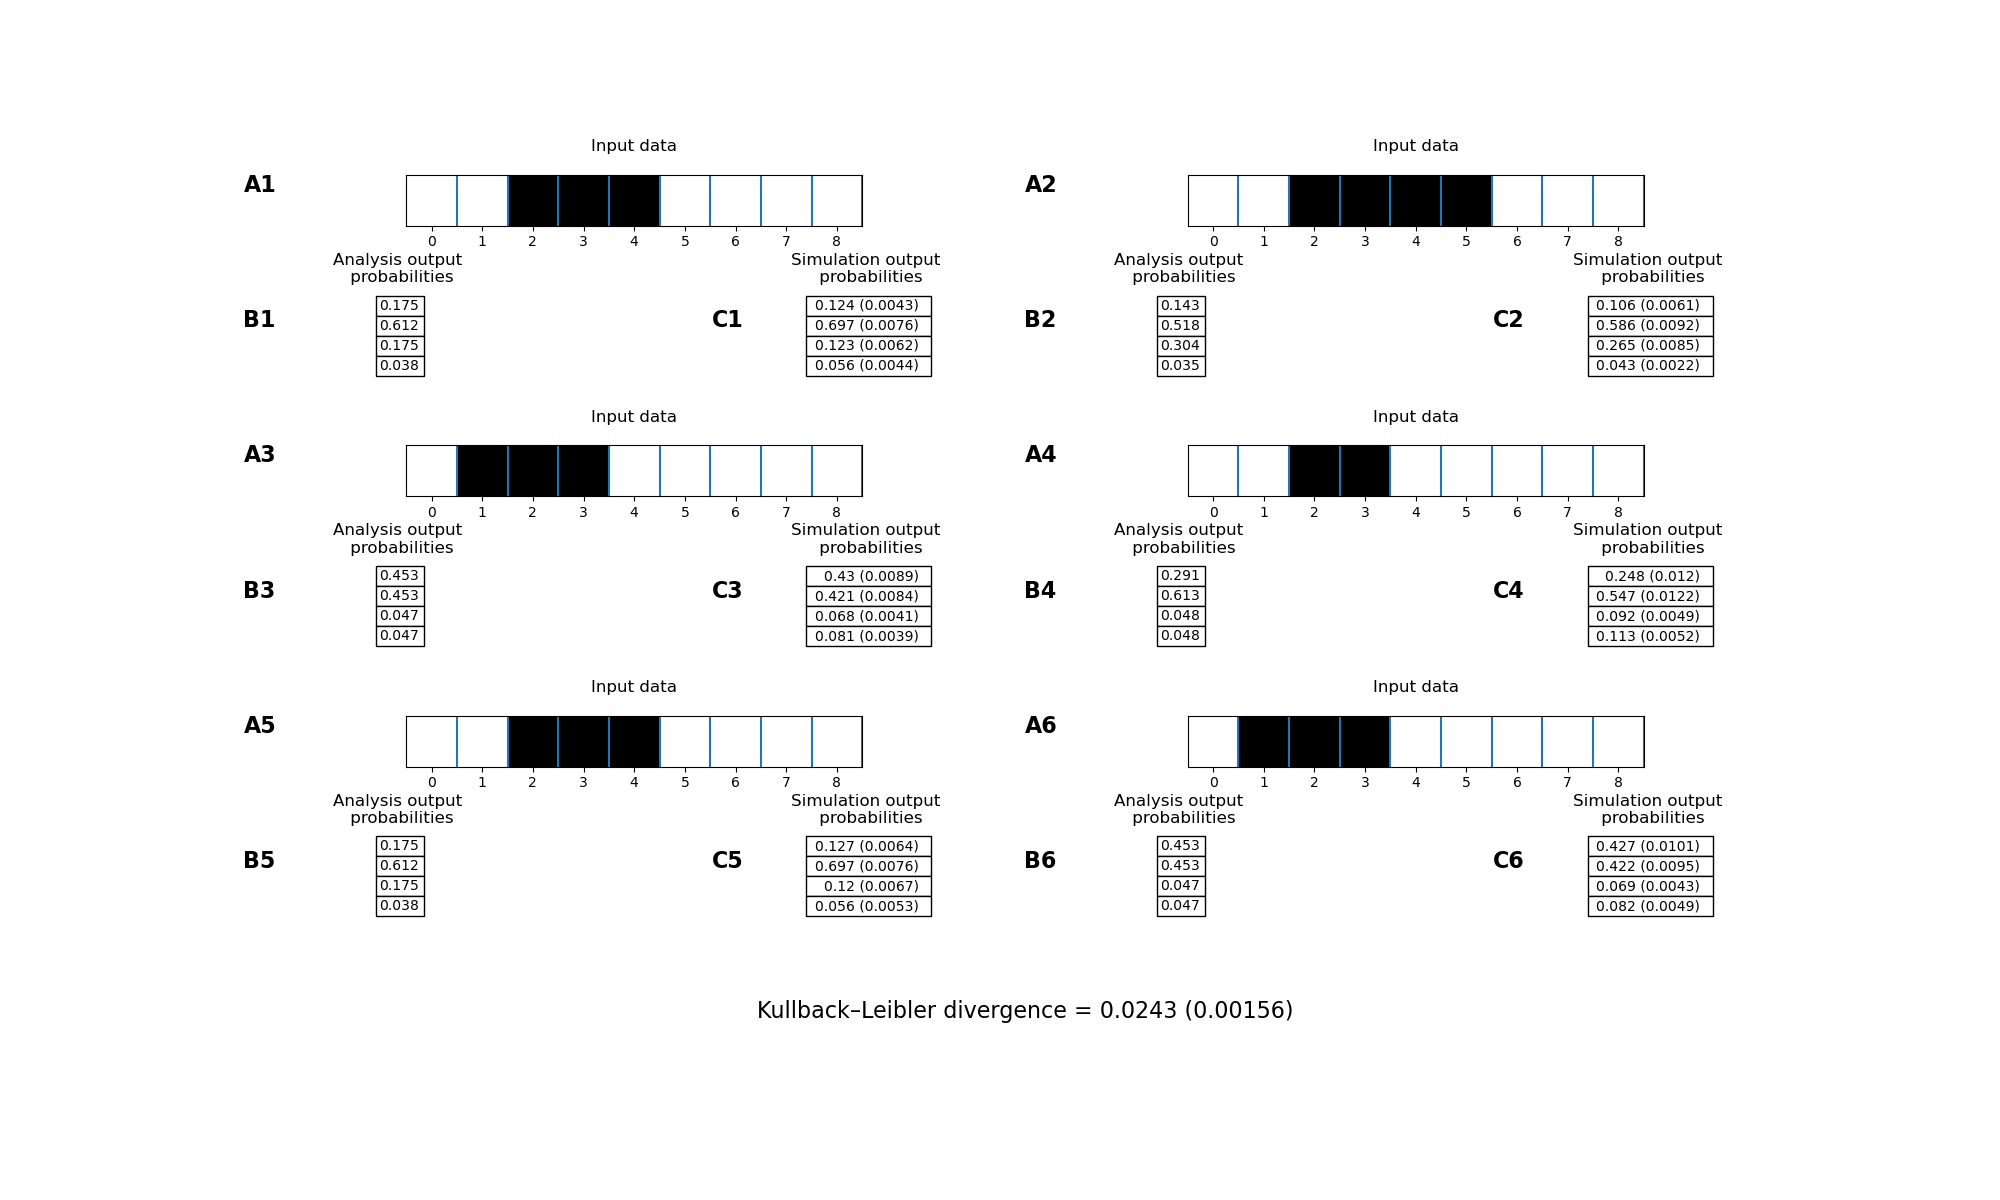
\includegraphics[width=\linewidth]{figures/1D/1D_42_0_15.png}
  \caption{\textbf{Analysis and simulation result. } Hyperparameters: $f_{input} = 42 Hz, f_{prior} = 0 Hz, \tau_{decay} = 15 ms$ \textbf{A} Input images with 9 x 1 pixels. \textbf{B} Analytically calculated posterior probabilities and simulated posterior probabilities. The standard deviations are given by the black bars.}
  \label{fig:1D_42_0_15}
\end{figure}

\begin{table}[]
\label{tab:1D_42_0_15}
\small
\tabcolsep=0.11cm
\begin{tabular}{|c|cc|cc|}
\hline
                       & \multicolumn{2}{c|}{Image 1}                       & \multicolumn{2}{c|}{Image 2}                       \\ \hline
                       & \multicolumn{1}{c|}{Analysis} & Simulation         & \multicolumn{1}{c|}{Analysis} & Simulation         \\ \hline
$y_0$                  & \multicolumn{1}{c|}{0.175}    & 0.124 $\pm$ 0.0061 & \multicolumn{1}{c|}{0.143}    & 0.104 $\pm$ 0.0059 \\ \hline
$y_1$                  & \multicolumn{1}{c|}{0.612}    & 0.699 $\pm$ 0.0093 & \multicolumn{1}{c|}{0.518}    & 0.587 $\pm$ 0.0090 \\ \hline
$y_2$                  & \multicolumn{1}{c|}{0.175}    & 0.121 $\pm$ 0.0058 & \multicolumn{1}{c|}{0.304}    & 0.266 $\pm$ 0.0067 \\ \hline
$y_3$                  & \multicolumn{1}{c|}{0.038}    & 0.056 $\pm$ 0.0033 & \multicolumn{1}{c|}{0.035}    & 0.043 $\pm$ 0.0025 \\ \hline
                       & \multicolumn{2}{c|}{Image 3}                       & \multicolumn{2}{c|}{Image 4}                       \\ \hline
$y_0$                  & \multicolumn{1}{c|}{0.453}    & 0.430 $\pm$ 0.0089 & \multicolumn{1}{c|}{0.291}    & 0.245 $\pm$ 0.0065 \\ \hline
$y_1$                  & \multicolumn{1}{c|}{0.453}    & 0.421 $\pm$ 0.0073 & \multicolumn{1}{c|}{0.613}    & 0.553 $\pm$ 0.0072 \\ \hline
$y_2$                  & \multicolumn{1}{c|}{0.047}    & 0.070 $\pm$ 0.0045 & \multicolumn{1}{c|}{0.048}    & 0.090 $\pm$ 0.0045 \\ \hline
$y_3$                  & \multicolumn{1}{c|}{0.047}    & 0.080 $\pm$ 0.0042 & \multicolumn{1}{c|}{0.048}    & 0.111 $\pm$ 0.0053 \\ \hline
						& \multicolumn{2}{c|}{Image 5}                       & \multicolumn{2}{c|}{Image 6}                       \\ \hline
$y_0$                  & \multicolumn{1}{c|}{0.175}    & 0.124 $\pm$ 0.0046 & \multicolumn{1}{c|}{0.453}    & 0.428 $\pm$ 0.0116 \\ \hline
$y_1$                  & \multicolumn{1}{c|}{0.612}    & 0.697 $\pm$ 0.0069 & \multicolumn{1}{c|}{0.453}    & 0.421 $\pm$ 0.0111 \\ \hline
$y_2$                  & \multicolumn{1}{c|}{0.175}    & 0.123 $\pm$ 0.0050 & \multicolumn{1}{c|}{0.047}    & 0.070 $\pm$ 0.0034 \\ \hline
$y_3$                  & \multicolumn{1}{c|}{0.038}    & 0.056 $\pm$ 0.0043 & \multicolumn{1}{c|}{0.047}    & 0.081 $\pm$ 0.0047 \\ \hline
\end{tabular}
\caption{\textbf{Analysis and simulation output probabilities. } Hyperparameters: $f_{input} = 42 Hz, f_{prior} = 0 Hz, \tau_{decay} = 15 ms$}
\end{table}

When $f_{input}$ was 70 Hz the results of the analysis and the simulation differed more as can be seen in Figure \ref{fig:1D_70_0_15} and Table \ref{tab:1D_70_0_15}.

\begin{figure}
  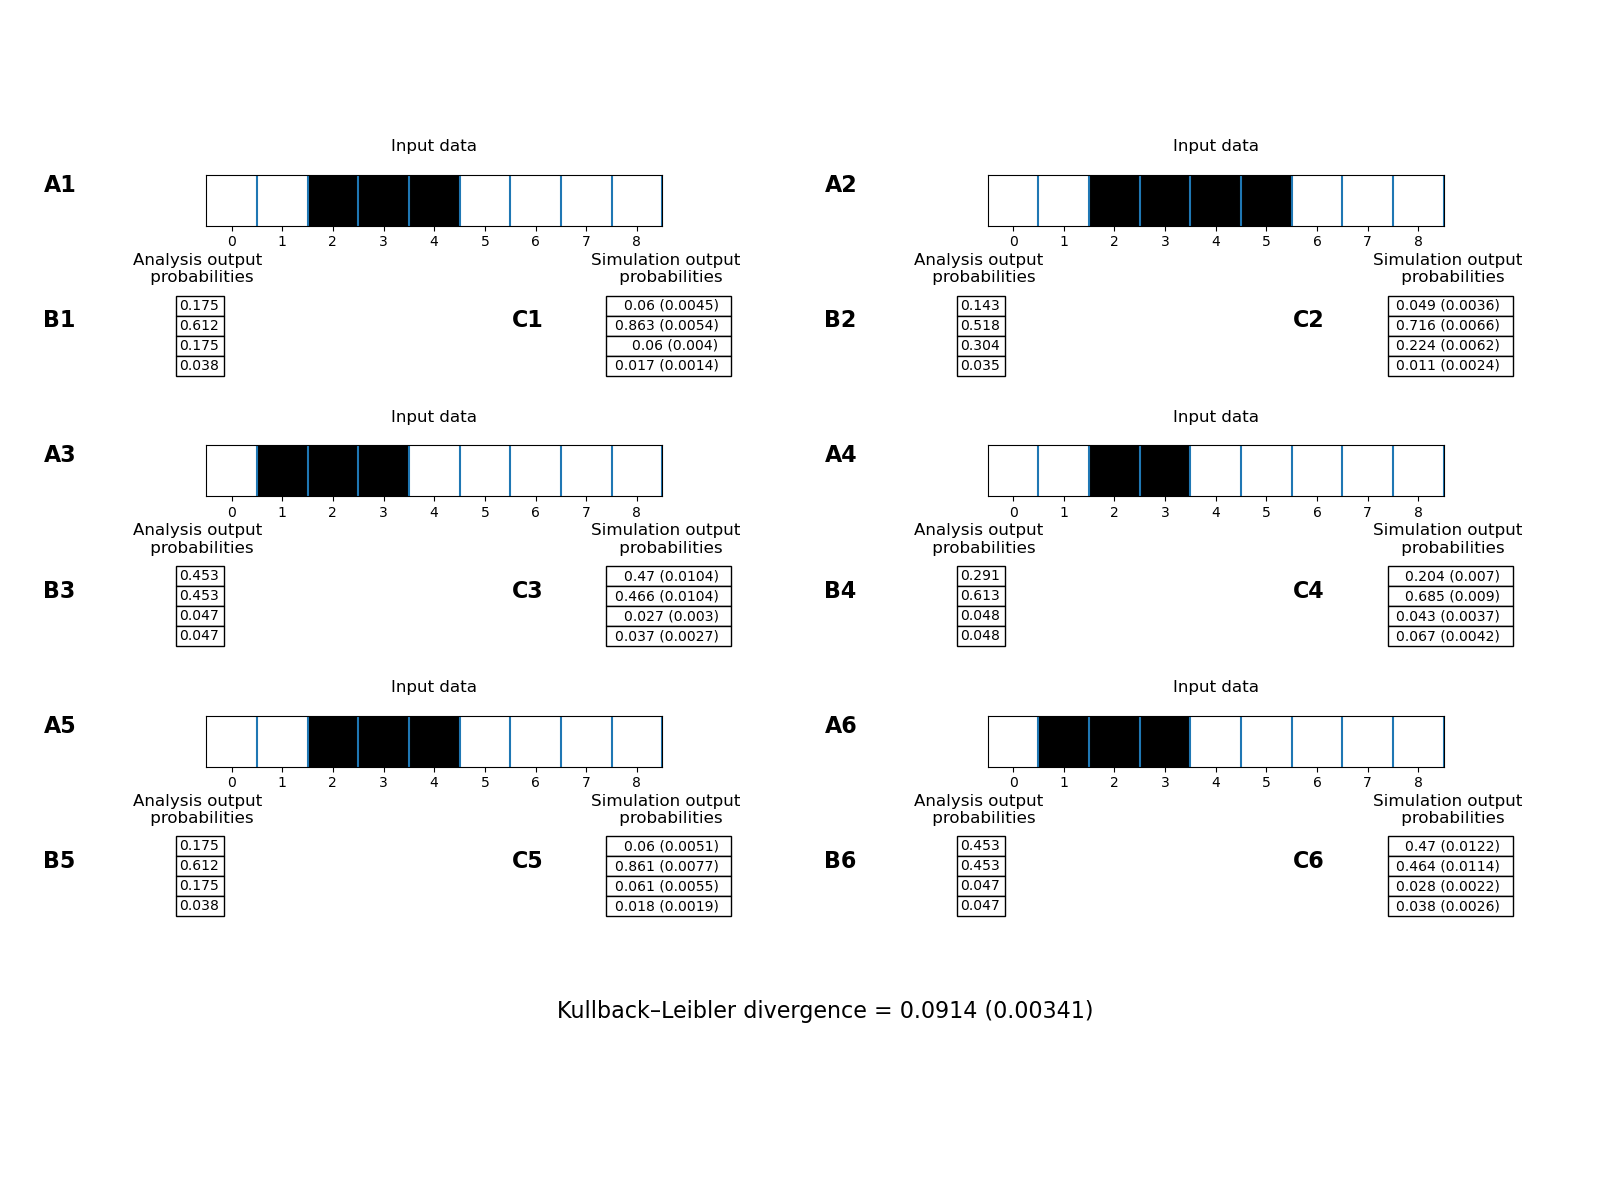
\includegraphics[width=\linewidth]{figures/1D/1D_70_0_15.png}
    \caption{\textbf{Analysis and simulation result. } Hyperparameters: $f_{input} = 70 Hz, f_{prior} = 0 Hz, \tau_{decay} = 15 ms$ \textbf{A} Input images with 9 x 1 pixels. \textbf{B} Analytically calculated posterior probabilities and simulated posterior probabilities. The standard deviations are given by the black bars.}
  \label{fig:1D_70_0_15}
\end{figure}

\begin{table}[]
\label{tab:1D_70_0_15}
\small
\tabcolsep=0.11cm
\begin{tabular}{|c|cc|cc|}
\hline
                       & \multicolumn{2}{c|}{Image 1}                       & \multicolumn{2}{c|}{Image 2}                       \\ \hline
                       & \multicolumn{1}{c|}{Analysis} & Simulation         & \multicolumn{1}{c|}{Analysis} & Simulation         \\ \hline
$y_0$                  & \multicolumn{1}{c|}{0.175}    & 0.061 $\pm$ 0.0038 & \multicolumn{1}{c|}{0.143}    & 0.049 $\pm$ 0.0027 \\ \hline
$y_1$                  & \multicolumn{1}{c|}{0.612}    & 0.861 $\pm$ 0.0065 & \multicolumn{1}{c|}{0.518}    & 0.715 $\pm$ 0.0083 \\ \hline
$y_2$                  & \multicolumn{1}{c|}{0.175}    & 0.061 $\pm$ 0.0041 & \multicolumn{1}{c|}{0.304}    & 0.226 $\pm$ 0.0070 \\ \hline
$y_3$                  & \multicolumn{1}{c|}{0.038}    & 0.017 $\pm$ 0.0016 & \multicolumn{1}{c|}{0.035}    & 0.011 $\pm$ 0.0017 \\ \hline
                       & \multicolumn{2}{c|}{Image 3}                       & \multicolumn{2}{c|}{Image 4}                       \\ \hline
$y_0$                  & \multicolumn{1}{c|}{0.453}    & 0.472 $\pm$ 0.0100 & \multicolumn{1}{c|}{0.291}    & 0.207 $\pm$ 0.0067 \\ \hline
$y_1$                  & \multicolumn{1}{c|}{0.453}    & 0.464 $\pm$ 0.0101 & \multicolumn{1}{c|}{0.613}    & 0.685 $\pm$ 0.0080 \\ \hline
$y_2$                  & \multicolumn{1}{c|}{0.047}    & 0.027 $\pm$ 0.0027 & \multicolumn{1}{c|}{0.048}    & 0.043 $\pm$ 0.0037 \\ \hline
$y_3$                  & \multicolumn{1}{c|}{0.047}    & 0.037 $\pm$ 0.0032 & \multicolumn{1}{c|}{0.048}    & 0.065 $\pm$ 0.0042 \\ \hline
						& \multicolumn{2}{c|}{Image 5}                       & \multicolumn{2}{c|}{Image 6}                       \\ \hline
$y_0$                  & \multicolumn{1}{c|}{0.175}    & 0.061 $\pm$ 0.0033 & \multicolumn{1}{c|}{0.453}    & 0.475 $\pm$ 0.0086 \\ \hline
$y_1$                  & \multicolumn{1}{c|}{0.612}    & 0.864 $\pm$ 0.0062 & \multicolumn{1}{c|}{0.453}    & 0.459 $\pm$ 0.0087 \\ \hline
$y_2$                  & \multicolumn{1}{c|}{0.175}    & 0.057 $\pm$ 0.0036 & \multicolumn{1}{c|}{0.047}    & 0.028 $\pm$ 0.0018 \\ \hline
$y_3$                  & \multicolumn{1}{c|}{0.038}    & 0.018 $\pm$ 0.0022 & \multicolumn{1}{c|}{0.047}    & 0.038 $\pm$ 0.0032 \\ \hline
\end{tabular}
\caption{\textbf{Analysis and simulation output probabilities. } Hyperparameters: $f_{input} = 70 Hz, f_{prior} = 0 Hz, \tau_{decay} = 15 ms$}
\end{table}

\subparagraph{$\tau_{decay} = 0.004 seconds$, $f_{prior} = 0 Hz$}
For this hyperparameter combination values between 50 and 150 Hz for $f_{input}$ in steps of 10 Hz were simulated. Analogously to the previous hyperparameter set after finding the best input firing rate the search was performed in finer steps until the best value was found at 88 Hz. The result of this search can be seen in Figure \ref{fig:1D_KLD_fPrior0_tau4}. The result of the simulation with those hyperparameters can be seen in Figure \ref{fig:1D_88_0_4} and Table \ref{tab:1D_88_0_4}.

\begin{figure}
\centering
  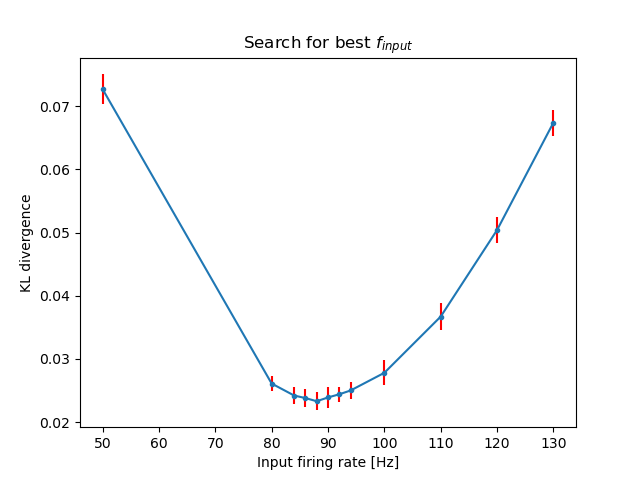
\includegraphics[width=0.75\linewidth]{figures/1D/KLDvsfInput_fPrior0tau4.png}
  \caption{\textbf{KL divergence for different $f_{input}$ values.} Hyperparameters: $f_{prior} = 0 Hz, \tau_{decay} = 4 ms$}
  \label{fig:1D_KLD_fPrior0_tau4}
\end{figure}

\begin{figure}
  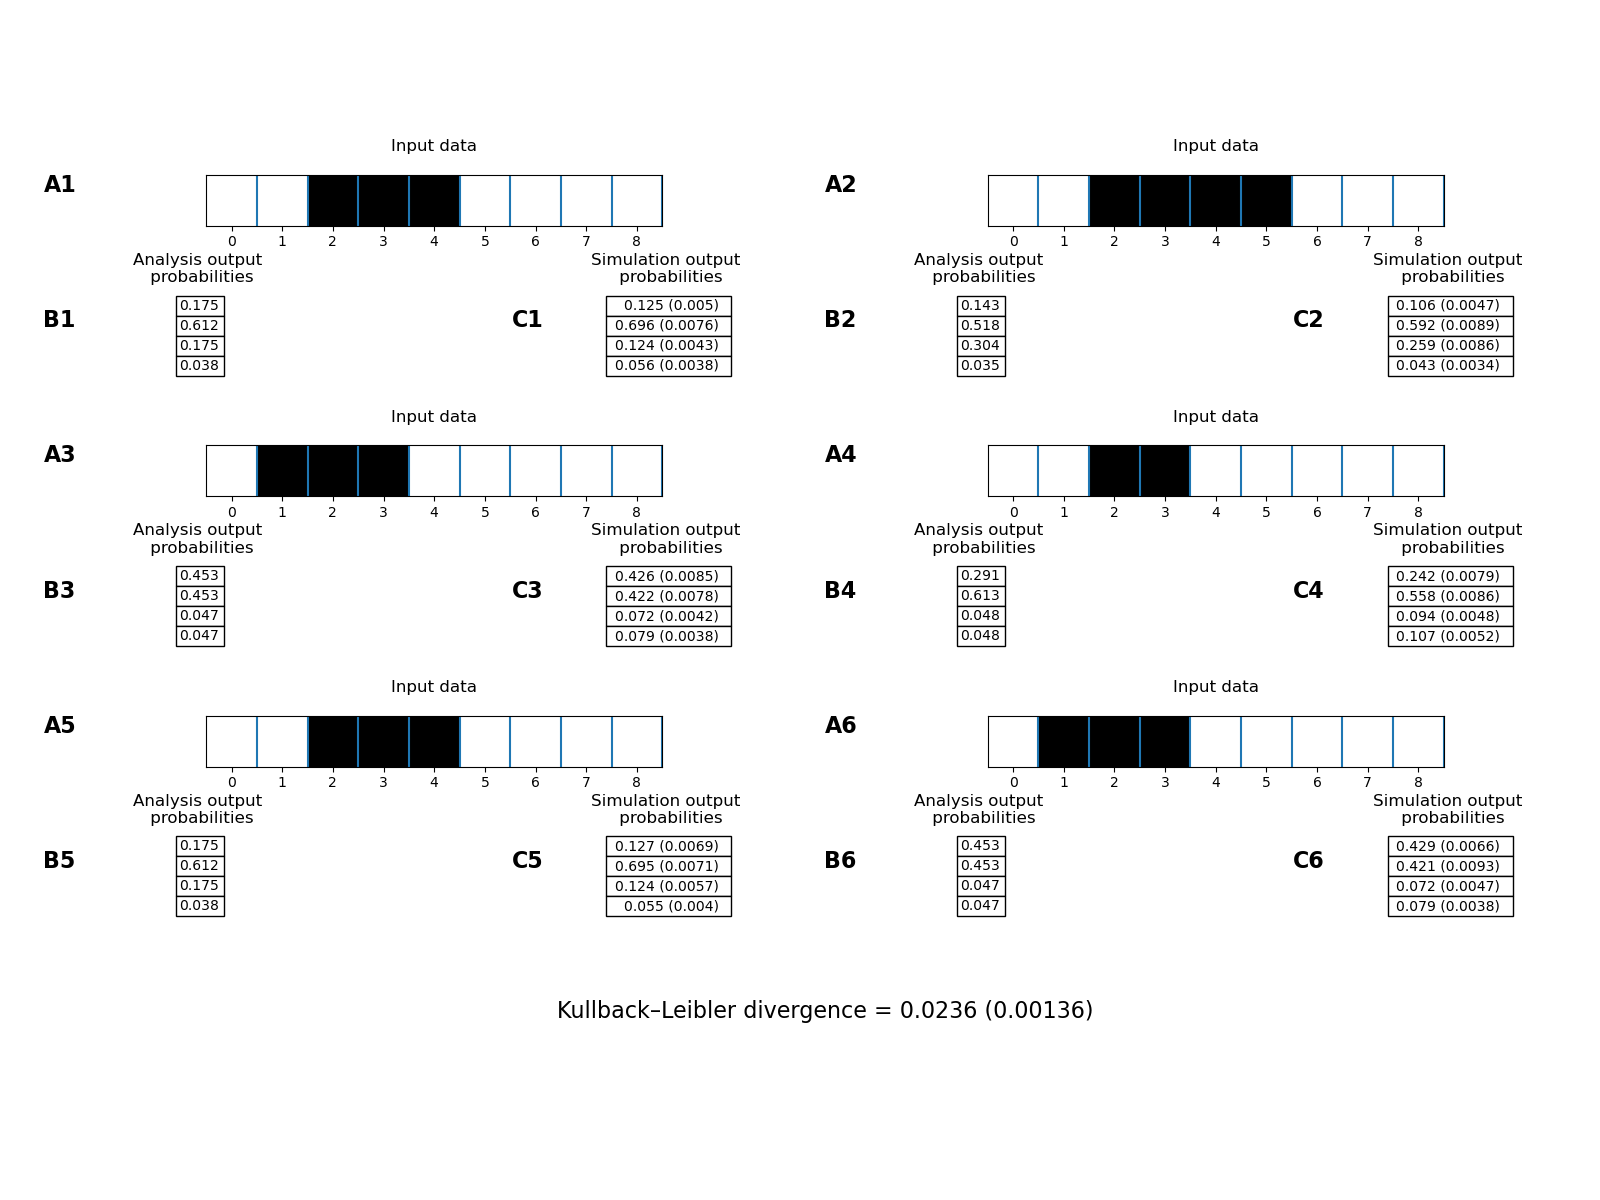
\includegraphics[width=\linewidth]{figures/1D/1D_88_0_4.png}
   \caption{\textbf{Analysis and simulation result. } Hyperparameters: $f_{input} = 88 Hz, f_{prior} = 0 Hz, \tau_{decay} = 4 ms$ \textbf{A} Input images with 9 x 1 pixels. \textbf{B} Analytically calculated posterior probabilities and simulated posterior probabilities. The standard deviations are given by the black bars.}
  \label{fig:1D_88_0_4}
\end{figure}

\begin{table}[]
\label{tab:1D_88_0_4}
\small
\tabcolsep=0.11cm
\begin{tabular}{|c|cc|cc|}
\hline
                       & \multicolumn{2}{c|}{Image 1}                       & \multicolumn{2}{c|}{Image 2}                       \\ \hline
                       & \multicolumn{1}{c|}{Analysis} & Simulation         & \multicolumn{1}{c|}{Analysis} & Simulation         \\ \hline
$y_0$                  & \multicolumn{1}{c|}{0.175}    & 0.126 $\pm$ 0.0050 & \multicolumn{1}{c|}{0.143}    & 0.106 $\pm$ 0.0054 \\ \hline
$y_1$                  & \multicolumn{1}{c|}{0.612}    & 0.695 $\pm$ 0.0066 & \multicolumn{1}{c|}{0.518}    & 0.587 $\pm$ 0.0098 \\ \hline
$y_2$                  & \multicolumn{1}{c|}{0.175}    & 0.124 $\pm$ 0.0049 & \multicolumn{1}{c|}{0.304}    & 0.264 $\pm$ 0.0072 \\ \hline
$y_3$                  & \multicolumn{1}{c|}{0.038}    & 0.054 $\pm$ 0.0039 & \multicolumn{1}{c|}{0.035}    & 0.043 $\pm$ 0.0028 \\ \hline
                       & \multicolumn{2}{c|}{Image 3}                       & \multicolumn{2}{c|}{Image 4}                       \\ \hline
$y_0$                  & \multicolumn{1}{c|}{0.453}    & 0.429 $\pm$ 0.0080 & \multicolumn{1}{c|}{0.291}    & 0.240 $\pm$ 0.0044 \\ \hline
$y_1$                  & \multicolumn{1}{c|}{0.453}    & 0.421 $\pm$ 0.0083 & \multicolumn{1}{c|}{0.613}    & 0.556 $\pm$ 0.0084 \\ \hline
$y_2$                  & \multicolumn{1}{c|}{0.047}    & 0.070 $\pm$ 0.0037 & \multicolumn{1}{c|}{0.048}    & 0.095 $\pm$ 0.0036 \\ \hline
$y_3$                  & \multicolumn{1}{c|}{0.047}    & 0.080 $\pm$ 0.0044 & \multicolumn{1}{c|}{0.048}    & 0.109 $\pm$ 0.0058 \\ \hline
						& \multicolumn{2}{c|}{Image 5}                       & \multicolumn{2}{c|}{Image 6}                       \\ \hline
$y_0$                  & \multicolumn{1}{c|}{0.175}    & 0.125 $\pm$ 0.0044 & \multicolumn{1}{c|}{0.453}    & 0.426 $\pm$ 0.0085 \\ \hline
$y_1$                  & \multicolumn{1}{c|}{0.612}    & 0.697 $\pm$ 0.0072 & \multicolumn{1}{c|}{0.453}    & 0.424 $\pm$ 0.0068 \\ \hline
$y_2$                  & \multicolumn{1}{c|}{0.175}    & 0.124 $\pm$ 0.0038 & \multicolumn{1}{c|}{0.047}    & 0.072 $\pm$ 0.0031 \\ \hline
$y_3$                  & \multicolumn{1}{c|}{0.038}    & 0.054 $\pm$ 0.0032 & \multicolumn{1}{c|}{0.047}    & 0.078 $\pm$ 0.0047 \\ \hline
\end{tabular}
\caption{\textbf{Analysis and simulation output probabilities. } Hyperparameters: $f_{input} = 88 Hz, f_{prior} = 0 Hz, \tau_{decay} = 4 ms$}
\end{table}

\paragraph{Simulation results with prior enabled}
After determining the best input firing rates for two different values of $\tau_{decay}$, the prior neurons were activated and the best $f_{prior}$ was searched.
\subparagraph{$\tau_{decay} = 0.015 seconds$, $f_{input} = 42 Hz$}
The search for the best value of $f_{prior}$ was performed in the same manner as for $f_{input}$. Values between 140 and 240 Hz were simulated and a prior firing rate of 222 Hz performed the best. The result of this search can be seen in Figure \ref{fig:1D_KLD_fInput42_tau15}. The simulation results can be seen in Figure \ref{fig:1D_42_222_15} and Table \ref{tab:1D_42_222_15}. In Figure \ref{fig:1D_42_222_15} the value of the prior is indicated by the red border which is three pixels wide and centered at the center position of the corresponding output class.

\begin{figure}
\centering
  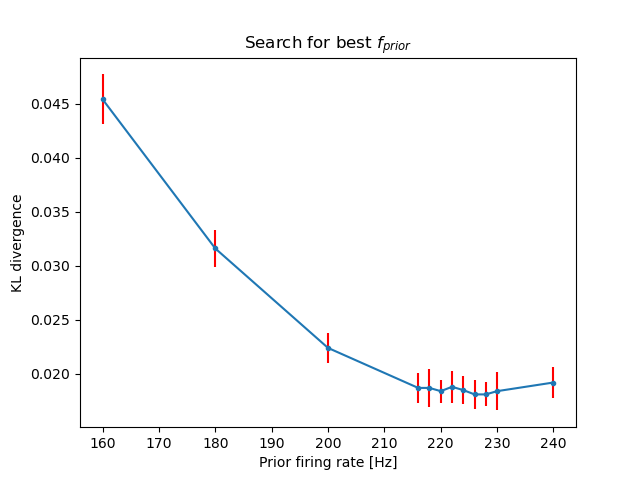
\includegraphics[width=0.75\linewidth]{figures/1D/KLDvsfPrior_fInput42tau15.png}
  \caption{\textbf{KL divergence for different $f_{prior}$ values.} Hyperparameters: $f_{input} = 42 Hz, \tau_{decay} = 15 ms$}
  \label{fig:1D_KLD_fInput42_tau15}
\end{figure}

\begin{figure}
  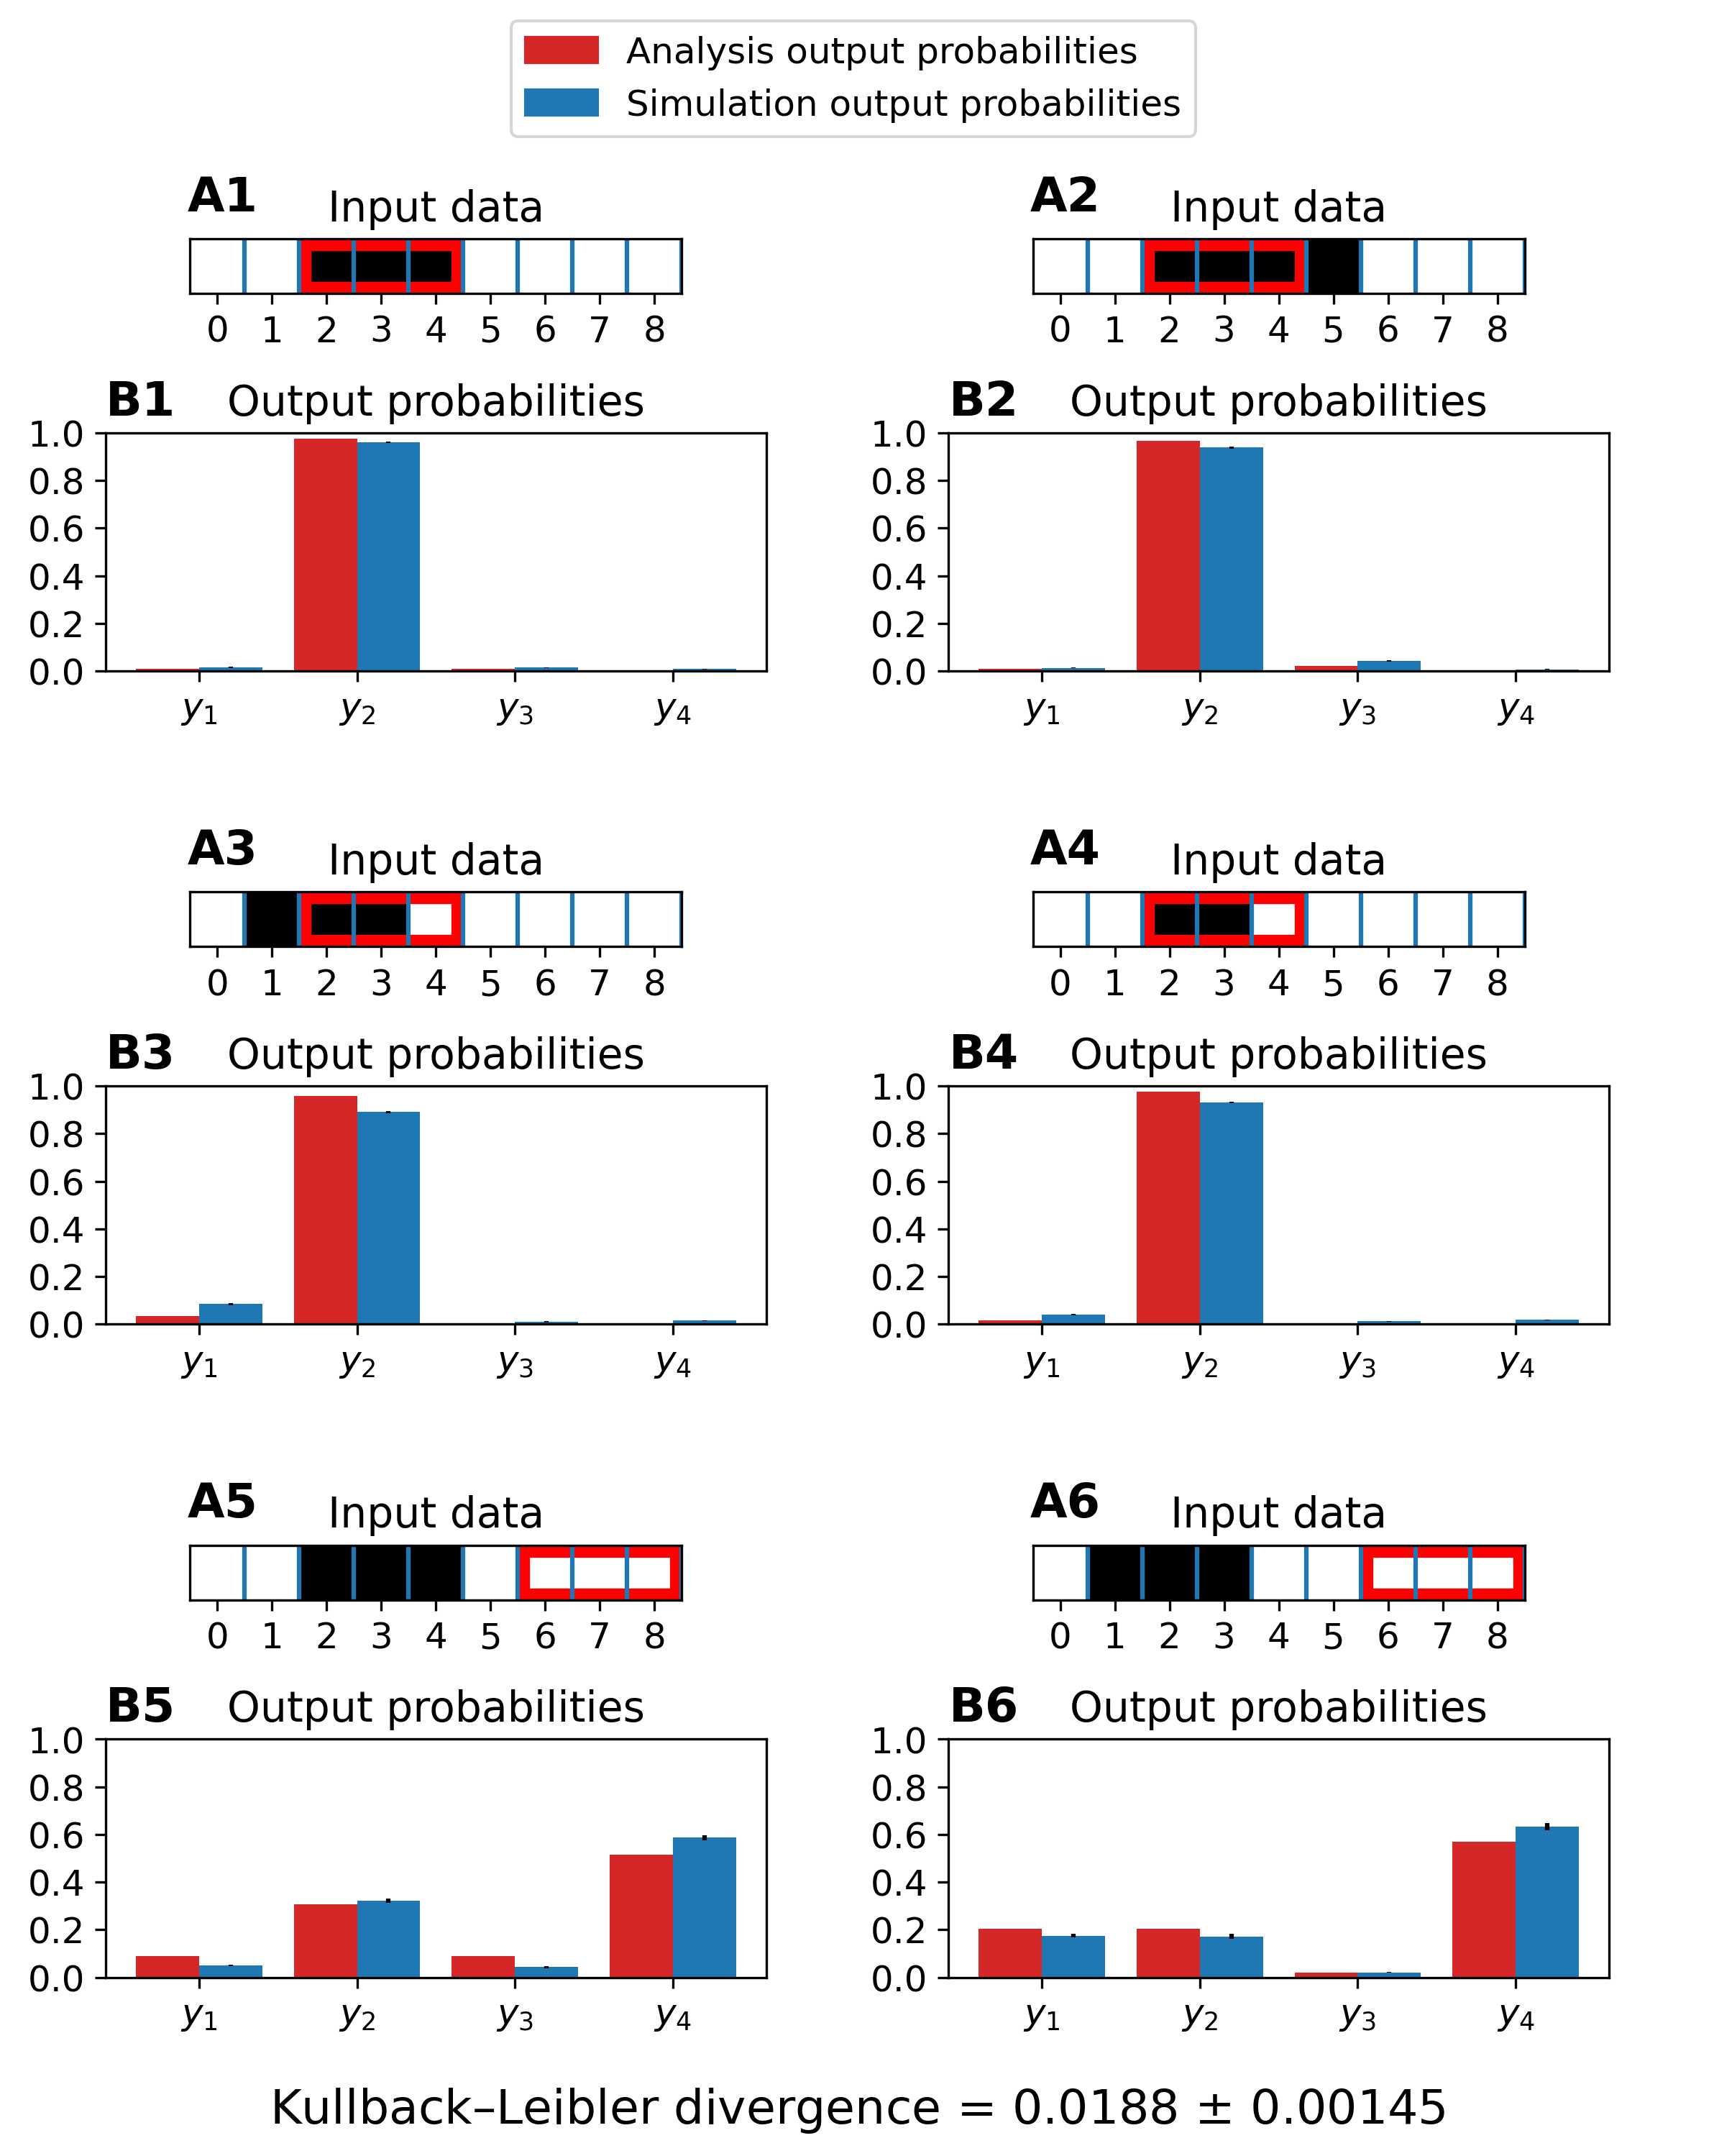
\includegraphics[width=\linewidth]{figures/1D/1D_42_222_15.png}
     \caption{\textbf{Analysis and simulation result. } Hyperparameters: $f_{input} = 42 Hz, f_{prior} = 222 Hz, \tau_{decay} = 15 ms$ \textbf{A} Input images with 9 x 1 pixels. Prior given as red border. \textbf{B} Analytically calculated posterior probabilities and simulated posterior probabilities. The standard deviations are given by the black bars.}
  \label{fig:1D_42_222_15}
\end{figure}

\begin{table}[]
\label{tab:1D_42_222_15}
\small
\tabcolsep=0.11cm
\begin{tabular}{|c|cc|cc|}
\hline
                       & \multicolumn{2}{c|}{Image 1}                       & \multicolumn{2}{c|}{Image 2}                       \\ \hline
                       & \multicolumn{1}{c|}{Analysis} & Simulation         & \multicolumn{1}{c|}{Analysis} & Simulation         \\ \hline
$y_0$                  & \multicolumn{1}{c|}{0.010}    & 0.015 $\pm$ 0.0021 & \multicolumn{1}{c|}{0.010}    & 0.013 $\pm$ 0.0016 \\ \hline
$y_1$                  & \multicolumn{1}{c|}{0.977}    & 0.962 $\pm$ 0.0030 & \multicolumn{1}{c|}{0.967}    & 0.938 $\pm$ 0.0040 \\ \hline
$y_2$                  & \multicolumn{1}{c|}{0.010}    & 0.015 $\pm$ 0.0017 & \multicolumn{1}{c|}{0.021}    & 0.042 $\pm$ 0.0032 \\ \hline
$y_3$                  & \multicolumn{1}{c|}{0.002}    & 0.008 $\pm$ 0.0016 & \multicolumn{1}{c|}{0.002}    & 0.007 $\pm$ 0.0013 \\ \hline
                       & \multicolumn{2}{c|}{Image 3}                       & \multicolumn{2}{c|}{Image 4}                       \\ \hline
$y_0$                  & \multicolumn{1}{c|}{0.035}    & 0.084 $\pm$ 0.0038 & \multicolumn{1}{c|}{0.017}    & 0.039 $\pm$ 0.0033 \\ \hline
$y_1$                  & \multicolumn{1}{c|}{0.957}    & 0.891 $\pm$ 0.0046 & \multicolumn{1}{c|}{0.977}    & 0.931 $\pm$ 0.0045 \\ \hline
$y_2$                  & \multicolumn{1}{c|}{0.004}    & 0.010 $\pm$ 0.0018 & \multicolumn{1}{c|}{0.003}    & 0.012 $\pm$ 0.0017 \\ \hline
$y_3$                  & \multicolumn{1}{c|}{0.004}    & 0.015 $\pm$ 0.0016 & \multicolumn{1}{c|}{0.003}    & 0.018 $\pm$ 0.0024 \\ \hline
						& \multicolumn{2}{c|}{Image 5}                       & \multicolumn{2}{c|}{Image 6}                       \\ \hline
$y_0$                  & \multicolumn{1}{c|}{0.088}    & 0.050 $\pm$ 0.0033 & \multicolumn{1}{c|}{0.205}    & 0.175 $\pm$ 0.0077 \\ \hline
$y_1$                  & \multicolumn{1}{c|}{0.308}    & 0.321 $\pm$ 0.0087 & \multicolumn{1}{c|}{0.205}    & 0.172 $\pm$ 0.0106 \\ \hline
$y_2$                  & \multicolumn{1}{c|}{0.088}    & 0.043 $\pm$ 0.0039 & \multicolumn{1}{c|}{0.021}    & 0.021 $\pm$ 0.0018 \\ \hline
$y_3$                  & \multicolumn{1}{c|}{0.515}    & 0.587 $\pm$ 0.0105 & \multicolumn{1}{c|}{0.570}    & 0.632 $\pm$ 0.0158 \\ \hline
\end{tabular}
\caption{\textbf{Analysis and simulation output probabilities. } Hyperparameters: $f_{input} = 42 Hz, f_{prior} = 222 Hz, \tau_{decay} = 15 ms$}
\end{table}

\subparagraph{$\tau_{decay} = 0.004 seconds$, $f_{input} = 88 Hz$}
The search for the best value of $f_{prior}$ was performed in the same manner as for $f_{input}$. Values between 360 and 460 Hz were simulated and a prior firing rate of 440 Hz performed the best. The result of this search can be seen in Figure \ref{fig:1D_KLD_fInput88_tau4}. The results of this hyperparameter combination are given in Figure \ref{fig:1D_88_440_4} and Table \ref{tab:1D_88_440_4}.

\begin{figure}
\centering
  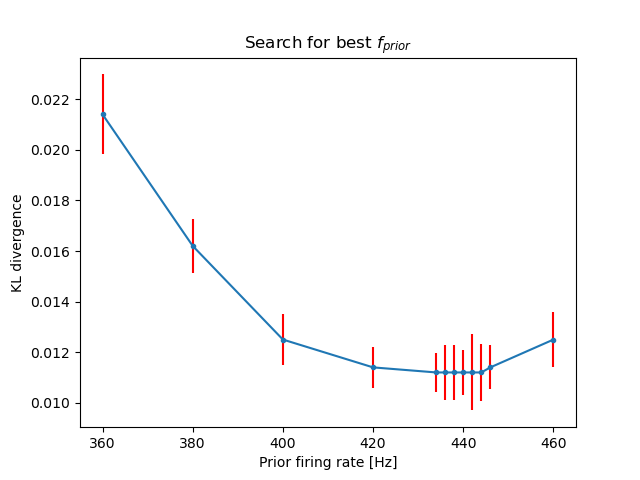
\includegraphics[width=0.75\linewidth]{figures/1D/KLDvsfPrior_fInput88tau4.png}
  \caption{\textbf{KL divergence for different $f_{prior}$ values.} Hyperparameters: $f_{input} = 88 Hz, \tau_{decay} = 4 ms$}
  \label{fig:1D_KLD_fInput88_tau4}
\end{figure}

\begin{figure}
  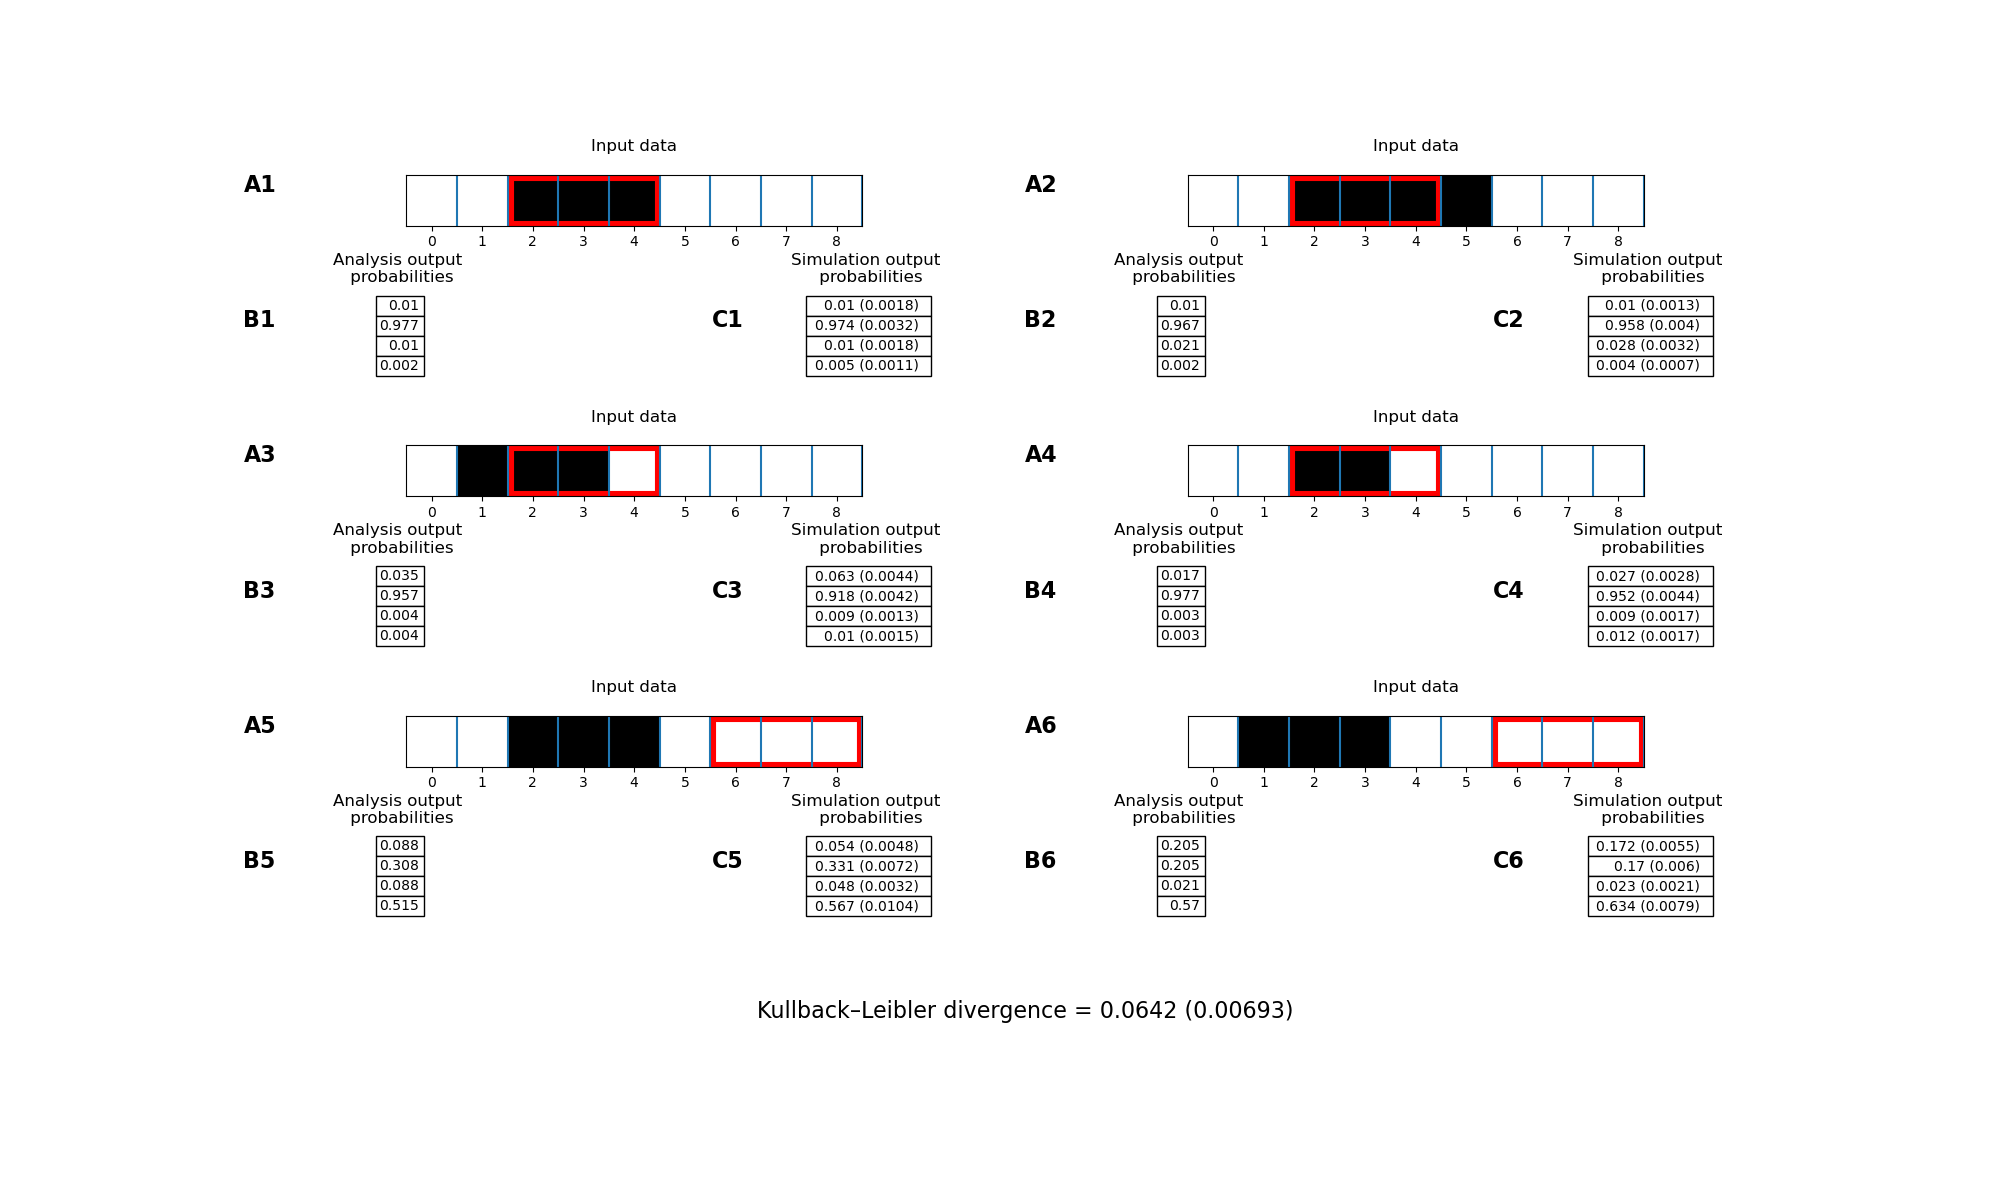
\includegraphics[width=\linewidth]{figures/1D/1D_88_440_4.png}
       \caption{\textbf{Analysis and simulation result. } Hyperparameters: $f_{input} = 88 Hz, f_{prior} = 440 Hz, \tau_{decay} = 4 ms$ \textbf{A} Input images with 9 x 1 pixels. Prior given as red border. \textbf{B} Analytically calculated posterior probabilities and simulated posterior probabilities. The standard deviations are given by the black bars.}
  \label{fig:1D_88_440_4}
\end{figure}

\begin{table}[]
\label{tab:1D_88_440_4}
\small
\tabcolsep=0.11cm
\begin{tabular}{|c|cc|cc|}
\hline
                       & \multicolumn{2}{c|}{Image 1}                       & \multicolumn{2}{c|}{Image 2}                       \\ \hline
                       & \multicolumn{1}{c|}{Analysis} & Simulation         & \multicolumn{1}{c|}{Analysis} & Simulation         \\ \hline
$y_0$                  & \multicolumn{1}{c|}{0.010}    & 0.011 $\pm$ 0.0016 & \multicolumn{1}{c|}{0.010}    & 0.010 $\pm$ 0.0017 \\ \hline
$y_1$                  & \multicolumn{1}{c|}{0.977}    & 0.974 $\pm$ 0.0026 & \multicolumn{1}{c|}{0.967}    & 0.957 $\pm$ 0.0034 \\ \hline
$y_2$                  & \multicolumn{1}{c|}{0.010}    & 0.010 $\pm$ 0.0019 & \multicolumn{1}{c|}{0.021}    & 0.028 $\pm$ 0.0036 \\ \hline
$y_3$                  & \multicolumn{1}{c|}{0.002}    & 0.005 $\pm$ 0.0013 & \multicolumn{1}{c|}{0.002}    & 0.005 $\pm$ 0.0011 \\ \hline
                       & \multicolumn{2}{c|}{Image 3}                       & \multicolumn{2}{c|}{Image 4}                       \\ \hline
$y_0$                  & \multicolumn{1}{c|}{0.035}    & 0.066 $\pm$ 0.0031 & \multicolumn{1}{c|}{0.017}    & 0.026 $\pm$ 0.0030 \\ \hline
$y_1$                  & \multicolumn{1}{c|}{0.957}    & 0.915 $\pm$ 0.0044 & \multicolumn{1}{c|}{0.977}    & 0.952 $\pm$ 0.0039 \\ \hline
$y_2$                  & \multicolumn{1}{c|}{0.004}    & 0.009 $\pm$ 0.0014 & \multicolumn{1}{c|}{0.003}    & 0.009 $\pm$ 0.0017 \\ \hline
$y_3$                  & \multicolumn{1}{c|}{0.004}    & 0.011 $\pm$ 0.0018 & \multicolumn{1}{c|}{0.003}    & 0.012 $\pm$ 0.0020 \\ \hline
						& \multicolumn{2}{c|}{Image 5}                       & \multicolumn{2}{c|}{Image 6}                       \\ \hline
$y_0$                  & \multicolumn{1}{c|}{0.088}    & 0.052 $\pm$ 0.0027 & \multicolumn{1}{c|}{0.205}    & 0.172 $\pm$ 0.0061 \\ \hline
$y_1$                  & \multicolumn{1}{c|}{0.308}    & 0.328 $\pm$ 0.0085 & \multicolumn{1}{c|}{0.205}    & 0.174 $\pm$ 0.0059 \\ \hline
$y_2$                  & \multicolumn{1}{c|}{0.088}    & 0.046 $\pm$ 0.0031 & \multicolumn{1}{c|}{0.021}    & 0.025 $\pm$ 0.0025 \\ \hline
$y_3$                  & \multicolumn{1}{c|}{0.515}    & 0.573 $\pm$ 0.0089 & \multicolumn{1}{c|}{0.570}    & 0.630 $\pm$ 0.0095 \\ \hline
\end{tabular}
\caption{\textbf{Analysis and simulation output probabilities. } Hyperparameters: $f_{input} = 88 Hz, f_{prior} = 440 Hz, \tau_{decay} = 4 ms$}
\end{table}


To demonstrate the impact of rising $f_{prior}$ it was set to 600 Hz and the results can be seen in Figure \ref{fig:1D_88_600_4} and Table \ref{tab:1D_88_600_4}.

\begin{figure}
  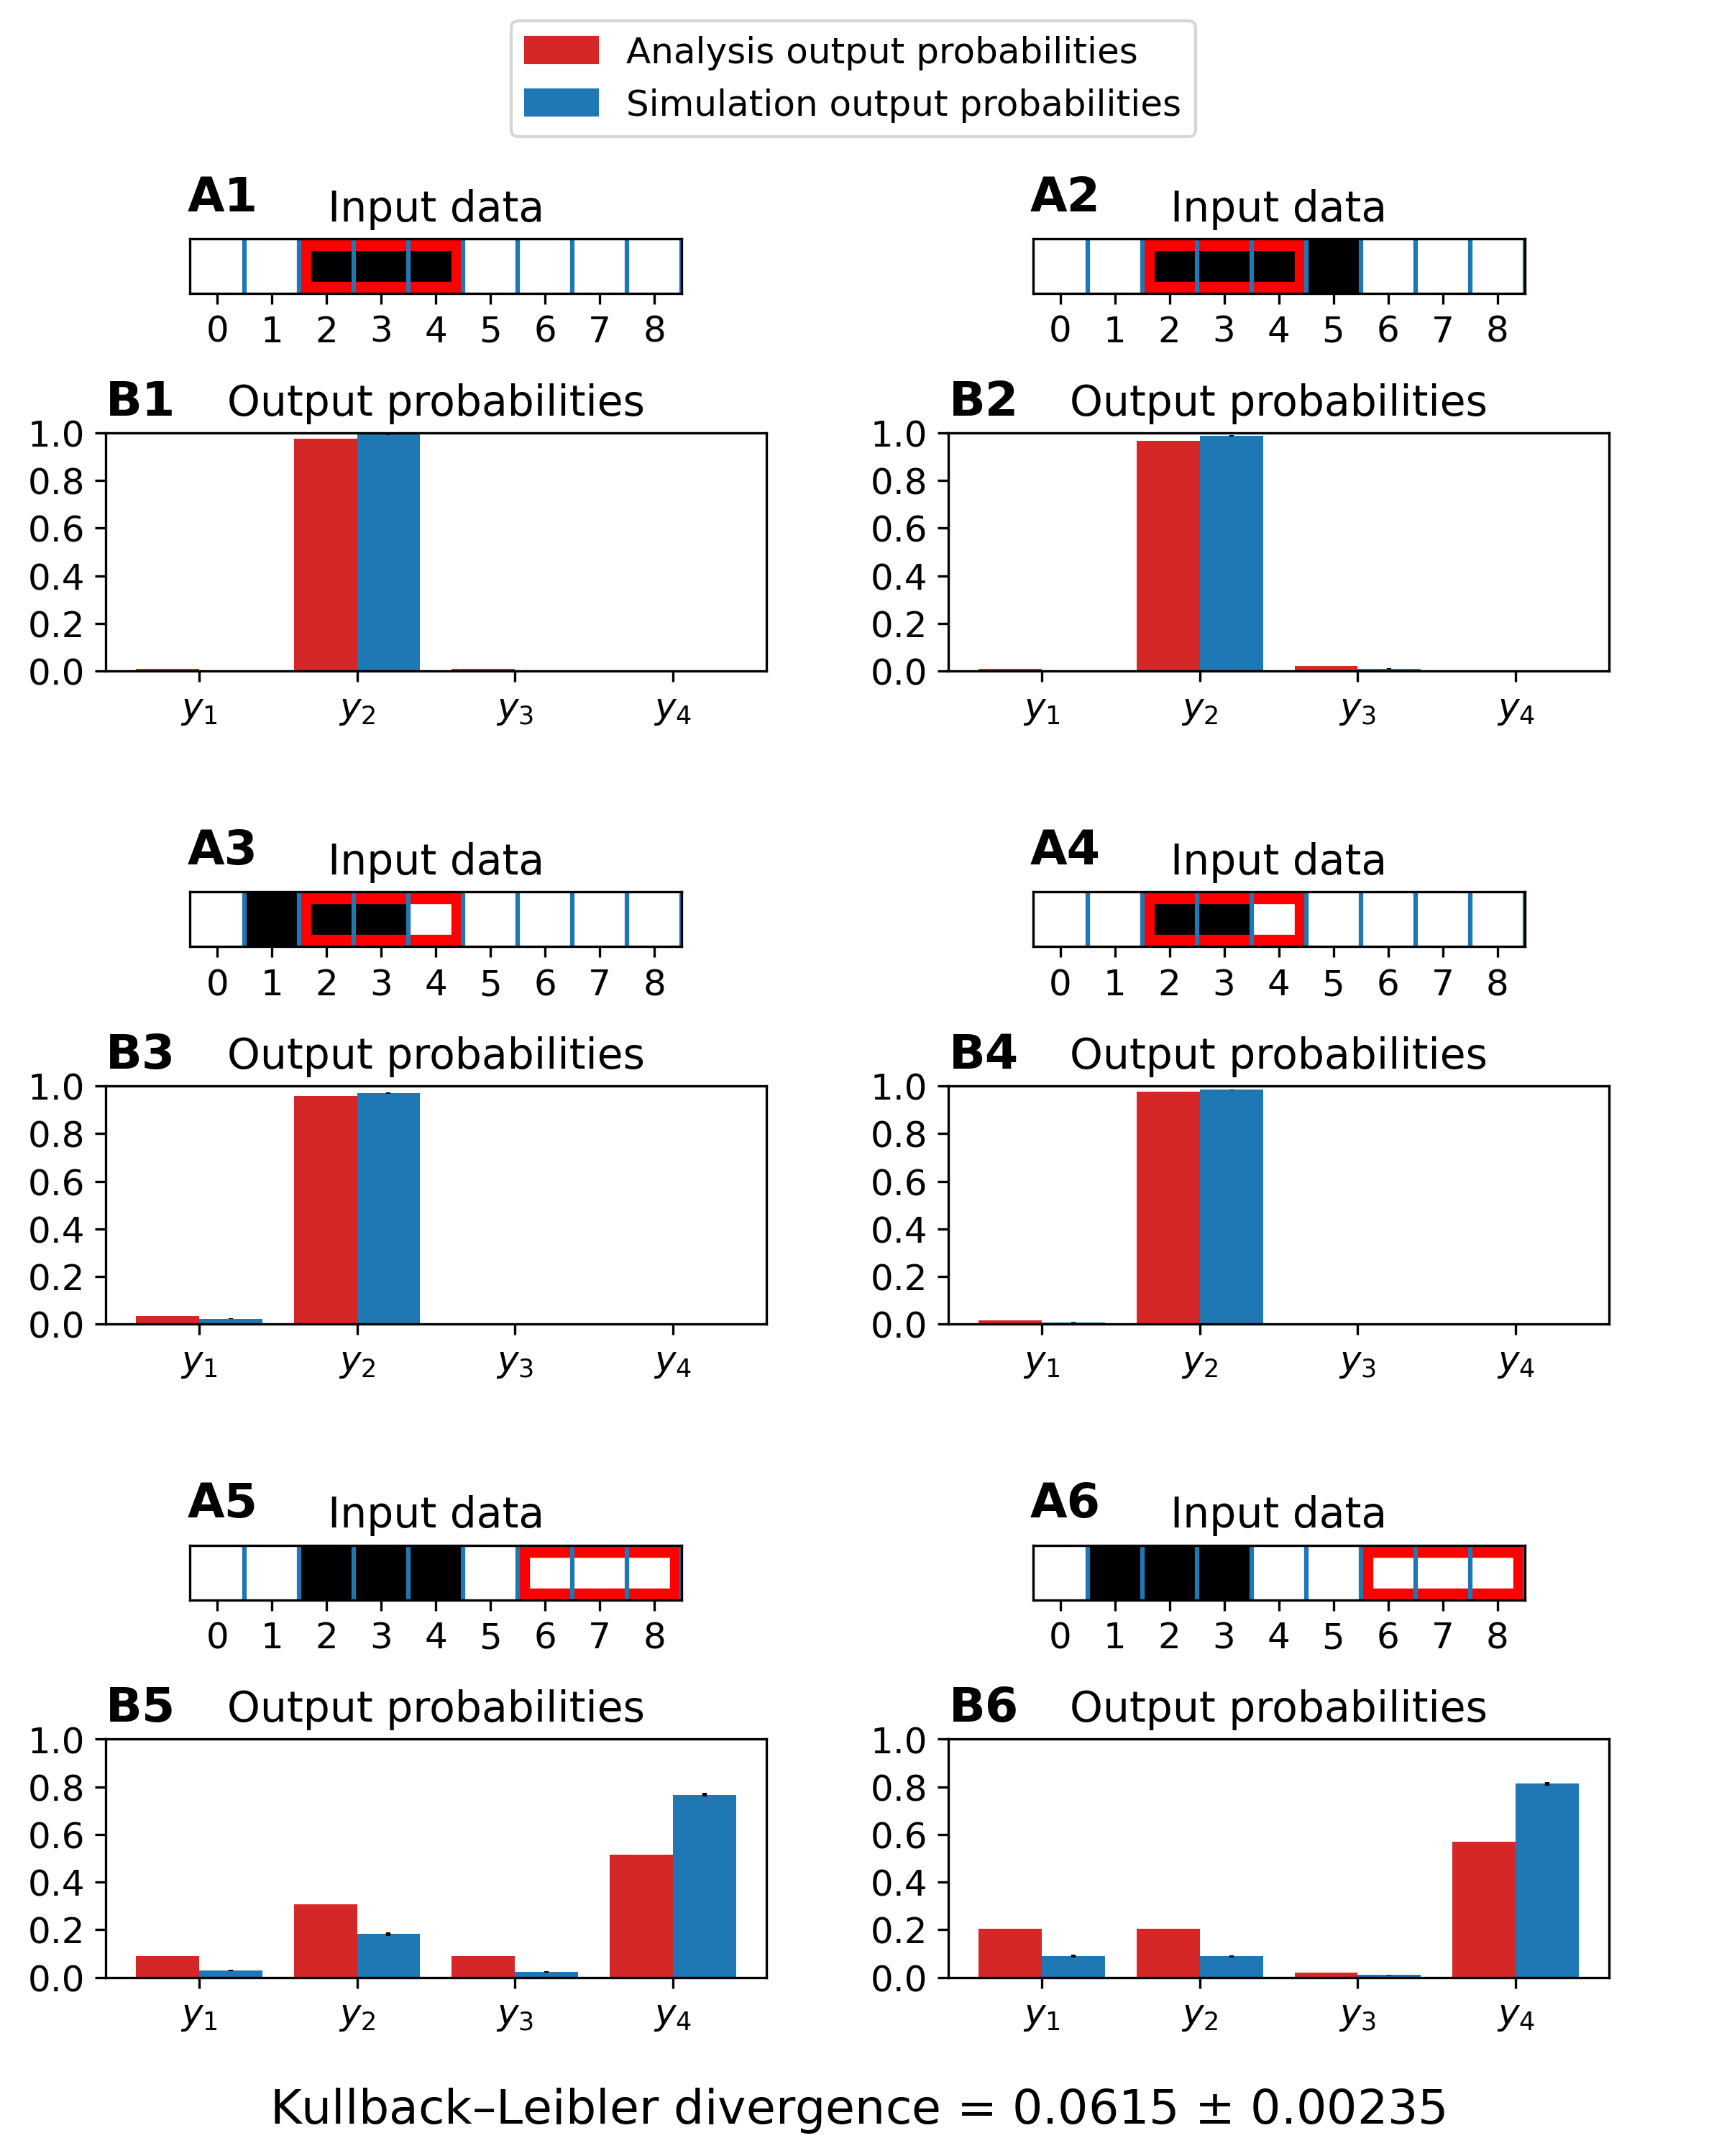
\includegraphics[width=\linewidth]{figures/1D/1D_88_600_4.png}
  \caption{\textbf{Analysis and simulation result. } Hyperparameters: $f_{input} = 88 Hz, f_{prior} = 600 Hz, \tau_{decay} = 4 ms$ \textbf{A} Input images with 9 x 1 pixels. Prior given as red border. \textbf{B} Analytically calculated posterior probabilities and simulated posterior probabilities. The standard deviations are given by the black bars.}
  \label{fig:1D_88_600_4}
\end{figure}

\begin{table}[]
\label{tab:1D_88_600_4}
\small
\tabcolsep=0.11cm
\begin{tabular}{|c|cc|cc|}
\hline
                       & \multicolumn{2}{c|}{Image 1}                       & \multicolumn{2}{c|}{Image 2}                       \\ \hline
                       & \multicolumn{1}{c|}{Analysis} & Simulation         & \multicolumn{1}{c|}{Analysis} & Simulation         \\ \hline
$y_0$                  & \multicolumn{1}{c|}{0.010}    & 0.003 $\pm$ 0.0011 & \multicolumn{1}{c|}{0.010}    & 0.003 $\pm$ 0.0009 \\ \hline
$y_1$                  & \multicolumn{1}{c|}{0.977}    & 0.993 $\pm$ 0.0013 & \multicolumn{1}{c|}{0.967}    & 0.987 $\pm$ 0.0024 \\ \hline
$y_2$                  & \multicolumn{1}{c|}{0.010}    & 0.003 $\pm$ 0.0008 & \multicolumn{1}{c|}{0.021}    & 0.009 $\pm$ 0.0019 \\ \hline
$y_3$                  & \multicolumn{1}{c|}{0.002}    & 0.001 $\pm$ 0.0005 & \multicolumn{1}{c|}{0.002}    & 0.001 $\pm$ 0.0008 \\ \hline
                       & \multicolumn{2}{c|}{Image 3}                       & \multicolumn{2}{c|}{Image 4}                       \\ \hline
$y_0$                  & \multicolumn{1}{c|}{0.035}    & 0.023 $\pm$ 0.0025 & \multicolumn{1}{c|}{0.017}    & 0.008 $\pm$ 0.0011 \\ \hline
$y_1$                  & \multicolumn{1}{c|}{0.957}    & 0.971 $\pm$ 0.0030 & \multicolumn{1}{c|}{0.977}    & 0.984 $\pm$ 0.0019 \\ \hline
$y_2$                  & \multicolumn{1}{c|}{0.004}    & 0.003 $\pm$ 0.0009 & \multicolumn{1}{c|}{0.003}    & 0.003 $\pm$ 0.0008 \\ \hline
$y_3$                  & \multicolumn{1}{c|}{0.004}    & 0.003 $\pm$ 0.0011 & \multicolumn{1}{c|}{0.003}    & 0.004 $\pm$ 0.0011 \\ \hline
						& \multicolumn{2}{c|}{Image 5}                       & \multicolumn{2}{c|}{Image 6}                       \\ \hline
$y_0$                  & \multicolumn{1}{c|}{0.088}    & 0.028 $\pm$ 0.0026 & \multicolumn{1}{c|}{0.205}    & 0.089 $\pm$ 0.0057 \\ \hline
$y_1$                  & \multicolumn{1}{c|}{0.308}    & 0.182 $\pm$ 0.0077 & \multicolumn{1}{c|}{0.205}    & 0.088 $\pm$ 0.0047 \\ \hline
$y_2$                  & \multicolumn{1}{c|}{0.088}    & 0.023 $\pm$ 0.0025 & \multicolumn{1}{c|}{0.021}    & 0.010 $\pm$ 0.0016 \\ \hline
$y_3$                  & \multicolumn{1}{c|}{0.515}    & 0.766 $\pm$ 0.0079 & \multicolumn{1}{c|}{0.570}    & 0.813 $\pm$ 0.0081 \\ \hline
\end{tabular}
\caption{\textbf{Analysis and simulation output probabilities. } Hyperparameters: $f_{input} = 88 Hz, f_{prior} = 600 Hz, \tau_{decay} = 4 ms$}
\end{table}

\subparagraph{$\tau_{decay} = 0.004 seconds$, $f_{input} = 98$, $f_{prior} = 440 Hz$}
Finally, it was tested if a increase of $f_{input}$ might decrease the Kullback-Leibler divergence even further. The network was simulated with increasing values of $f_{input}$ in steps of 2 Hz, beginning from 90 Hz. The result of this search can be seen in Figure \ref{fig:1D_KLD_fPrior440_tau4}. The best result was obtained with an input firing rate of 98 Hz. The results of that simulation can be seen in Figure \ref{fig:1D_98_440_4} and Table \ref{tab:1D_98_440_4}.

\begin{figure}
\centering
  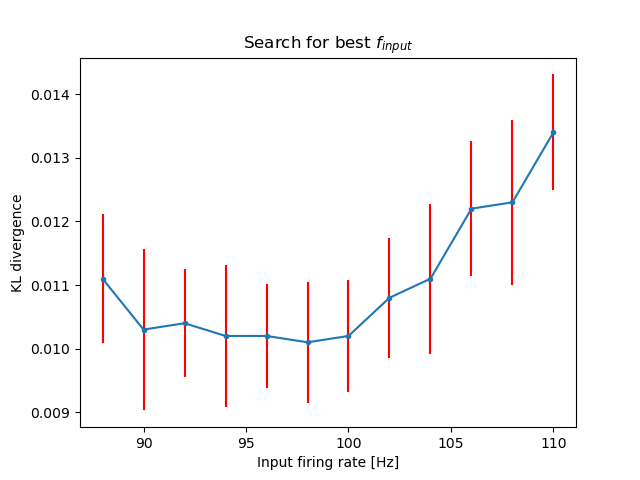
\includegraphics[width=0.75\linewidth]{figures/1D/KLDvsfInput_fPrior440tau4.png}
  \caption{\textbf{KL divergence for different $f_{input}$ values.} Hyperparameters: $f_{prior} = 440 Hz, \tau_{decay} = 4 ms$}
  \label{fig:1D_KLD_fPrior440_tau4}
\end{figure}

\begin{figure}
  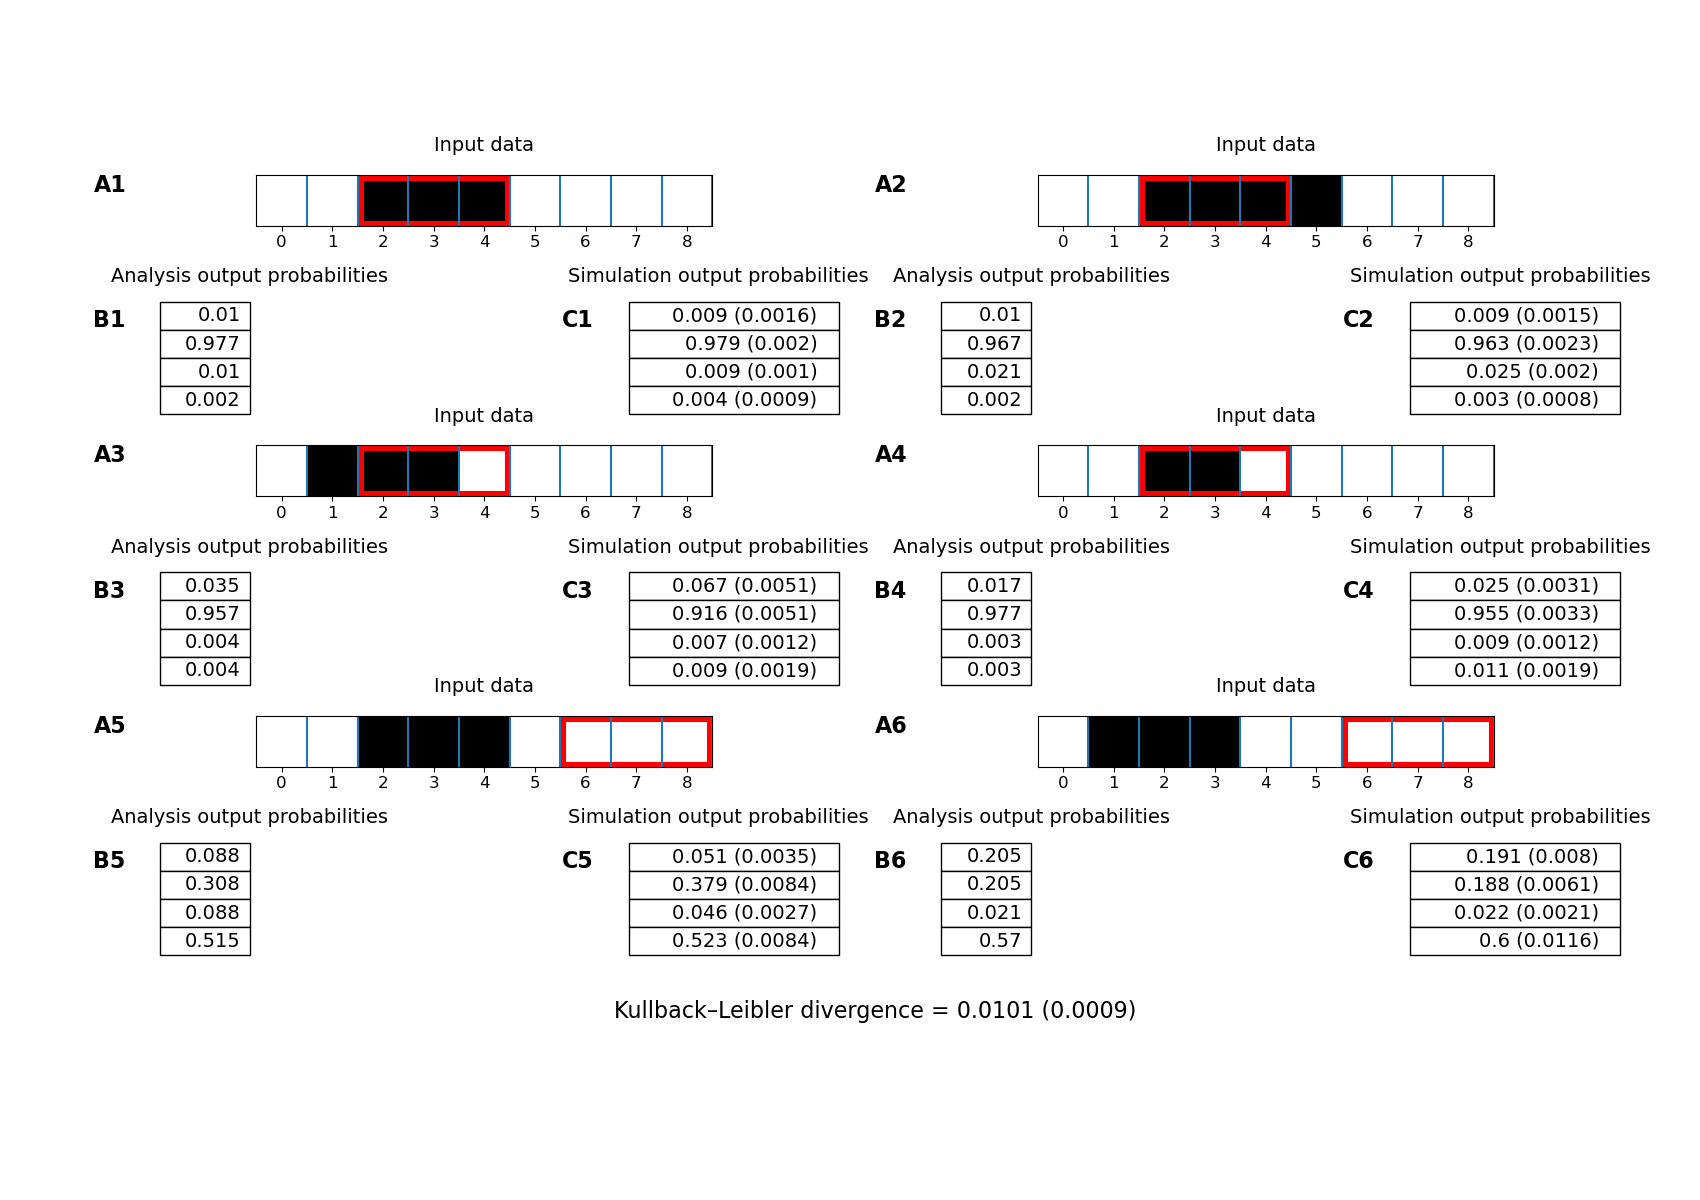
\includegraphics[width=\linewidth]{figures/1D/1D_98_440_4.png}
    \caption{\textbf{Analysis and simulation result. } Hyperparameters: $f_{input} = 98 Hz, f_{prior} = 440 Hz, \tau_{decay} = 4 ms$ \textbf{A} Input images with 9 x 1 pixels. Prior given as red border. \textbf{B} Analytically calculated posterior probabilities and simulated posterior probabilities. The standard deviations are given by the black bars.}
  \label{fig:1D_98_440_4}
\end{figure}

\begin{table}[]
\label{tab:1D_98_440_4}
\small
\tabcolsep=0.11cm
\begin{tabular}{|c|cc|cc|}
\hline
                       & \multicolumn{2}{c|}{Image 1}                       & \multicolumn{2}{c|}{Image 2}                       \\ \hline
                       & \multicolumn{1}{c|}{Analysis} & Simulation         & \multicolumn{1}{c|}{Analysis} & Simulation         \\ \hline
$y_0$                  & \multicolumn{1}{c|}{0.010}    & 0.009 $\pm$ 0.0016 & \multicolumn{1}{c|}{0.010}    & 0.009 $\pm$ 0.0015 \\ \hline
$y_1$                  & \multicolumn{1}{c|}{0.977}    & 0.979 $\pm$ 0.0020 & \multicolumn{1}{c|}{0.967}    & 0.963 $\pm$ 0.0023 \\ \hline
$y_2$                  & \multicolumn{1}{c|}{0.010}    & 0.009 $\pm$ 0.0010 & \multicolumn{1}{c|}{0.021}    & 0.025 $\pm$ 0.0020 \\ \hline
$y_3$                  & \multicolumn{1}{c|}{0.002}    & 0.004 $\pm$ 0.0009 & \multicolumn{1}{c|}{0.002}    & 0.003 $\pm$ 0.0008 \\ \hline
                       & \multicolumn{2}{c|}{Image 3}                       & \multicolumn{2}{c|}{Image 4}                       \\ \hline
$y_0$                  & \multicolumn{1}{c|}{0.035}    & 0.067 $\pm$ 0.0051 & \multicolumn{1}{c|}{0.017}    & 0.025 $\pm$ 0.0031 \\ \hline
$y_1$                  & \multicolumn{1}{c|}{0.957}    & 0.916 $\pm$ 0.0051 & \multicolumn{1}{c|}{0.977}    & 0.955 $\pm$ 0.0033 \\ \hline
$y_2$                  & \multicolumn{1}{c|}{0.004}    & 0.007 $\pm$ 0.0012 & \multicolumn{1}{c|}{0.003}    & 0.009 $\pm$ 0.0012 \\ \hline
$y_3$                  & \multicolumn{1}{c|}{0.004}    & 0.009 $\pm$ 0.0019 & \multicolumn{1}{c|}{0.003}    & 0.011 $\pm$ 0.0019 \\ \hline
						& \multicolumn{2}{c|}{Image 5}                       & \multicolumn{2}{c|}{Image 6}                       \\ \hline
$y_0$                  & \multicolumn{1}{c|}{0.088}    & 0.051 $\pm$ 0.0035 & \multicolumn{1}{c|}{0.205}    & 0.191 $\pm$ 0.0080 \\ \hline
$y_1$                  & \multicolumn{1}{c|}{0.308}    & 0.379 $\pm$ 0.0084 & \multicolumn{1}{c|}{0.205}    & 0.188 $\pm$ 0.0061 \\ \hline
$y_2$                  & \multicolumn{1}{c|}{0.088}    & 0.046 $\pm$ 0.0027 & \multicolumn{1}{c|}{0.021}    & 0.022 $\pm$ 0.0021 \\ \hline
$y_3$                  & \multicolumn{1}{c|}{0.515}    & 0.523 $\pm$ 0.0084 & \multicolumn{1}{c|}{0.570}    & 0.600 $\pm$ 0.0116 \\ \hline
\end{tabular}
\caption{\textbf{Analysis and simulation output probabilities. } Hyperparameters: $f_{input} = 98 Hz, f_{prior} = 440 Hz, \tau_{decay} = 4 ms$}
\end{table}

\paragraph{Approximating the analytic solution}
After first finding the optimal $f_{input}$ for disabled prior activity and then finding the optimal $f_{prior}$ with enabled prior activity for $\tau_{decay}$ the simulation was not yet approximating the analytical solution perfectly. Because of that it was tried to raise $f_{input}$ to further decrease the Kullback-Leibler divergence. The further search for a better $f_{input}$ was performed for $\tau_{decay} = 0.004 ms$ and $f_{prior} = 440 Hz$, as this set of hyperparameters performed the best overall.
When comparing the former optimal result in Figure \ref{fig:1D_88_440_4} with $f_{input} = 88 Hz$, to the result with $f_{input} = 98 Hz$ in Figure \ref{fig:1D_98_440_4}, it can be seen that the Kullback-Leibler divergence decreased from 0.0112 to 0.0101. However, when comparing Tables \ref{tab:1D_88_440_4} and \ref{tab:1D_98_440_4}, it can be seen that the higher $f_{input}$ did not perform strictly better. The simulation output probabilities for Image 3 improved, while for Image 5 the output probability of $y_2$ diverged more. A further increase of $f_{input}$ started to increase the Kullback-Leibler divergence again, thus the final optimum of the hyperparameter set was reached. It was assumed that increasing $f_{input}$ after $f_{prior}$ was fitted was necessary because the overall impact of $f_{input}$ on the simulation decreased due to the introduction of the prior activity.

\section{Experiment 3: Transferability of hyperparameters}
\label{section:1DDoubleSize}

\subsection{Introduction}
In this experiment the optimal hyperparameters determined in Experiment 2 were used, while doubling the size of the network and input images of Experiment 2. The goal was to determine if the hyperparameters are universally applicable, regardless of the network size.

\subsection{Methods}
The number input neurons was doubled from 18 to 36 neurons. This resulted in input images with 18 pixels. To double the effect of the prior neurons $f_{prior}$ was doubled to 880 Hz, while the amount of the prior neurons was kept the same with 4 prior neurons. Furthermore the matrix $P^{X|Y}$ was doubled in size by copying each value of the matrix to the right of itself.  The rest of the methods were performed analogously to Experiment 2.

\subsection{Results}

The expanded matrix $P^{X|Y}$ had its columns doubled, resulting in a dimension of $[18 \times 4]$. This yielded

\setcounter{MaxMatrixCols}{18}

\begin{equation}
\footnotesize
\label{eqn:pXvorausgesetztYResultDoubled}
\begin{matrix}
P^{X|Y} = \\
\begin{bmatrix}
0.9 & 0.9 & 0.9 & 0.9 & 0.9 & 0.9 & 0.1 & 0.1 & 0.1 & 0.1 & 0.1 & 0.1 & 0.1 & 0.1 & 0.1 & 0.1 & 0.1 & 0.1\\
0.1 & 0.1 & 0.1 & 0.1 & 0.9 & 0.9 & 0.9 & 0.9 & 0.9 & 0.9 & 0.1 & 0.1 & 0.1 & 0.1 & 0.1 & 0.1 & 0.1 & 0.1\\
0.1 & 0.1 & 0.1 & 0.1 & 0.1 & 0.1 & 0.1 & 0.1 & 0.9 & 0.9 & 0.9 & 0.9 & 0.9 & 0.9 & 0.1 & 0.1 & 0.1 & 0.1\\
0.1 & 0.1 & 0.1 & 0.1 & 0.1 & 0.1 & 0.1 & 0.1 & 0.1 & 0.1 & 0.1 & 0.1 & 0.9 & 0.9 & 0.9 & 0.9 & 0.9 & 0.9\\
\end{bmatrix}.
\end{matrix}
\end{equation}

The simulation result for $f_{input} = 98 Hz$, $f_{prior} = 880 Hz$ and $\tau_{decay} = 4 ms$ can be seen in Figure \ref{fig:doubleSize_98_880_4} and Table \ref{tab:doubleSize_98_880_4}. Initially the Kullback-Leibler divergence was infinite in this result, because some simulation output probabilities were zero and the Kullback-Leibler divergence is not defined for probabilities of zero. To circumvent this an approximated Kullback-Leibler divergence was calculated by setting the simulation output probabilities that were 0 to 0.0000001. This yielded a Kullback-Leibler divergence of 0.2392.
\begin{figure}
  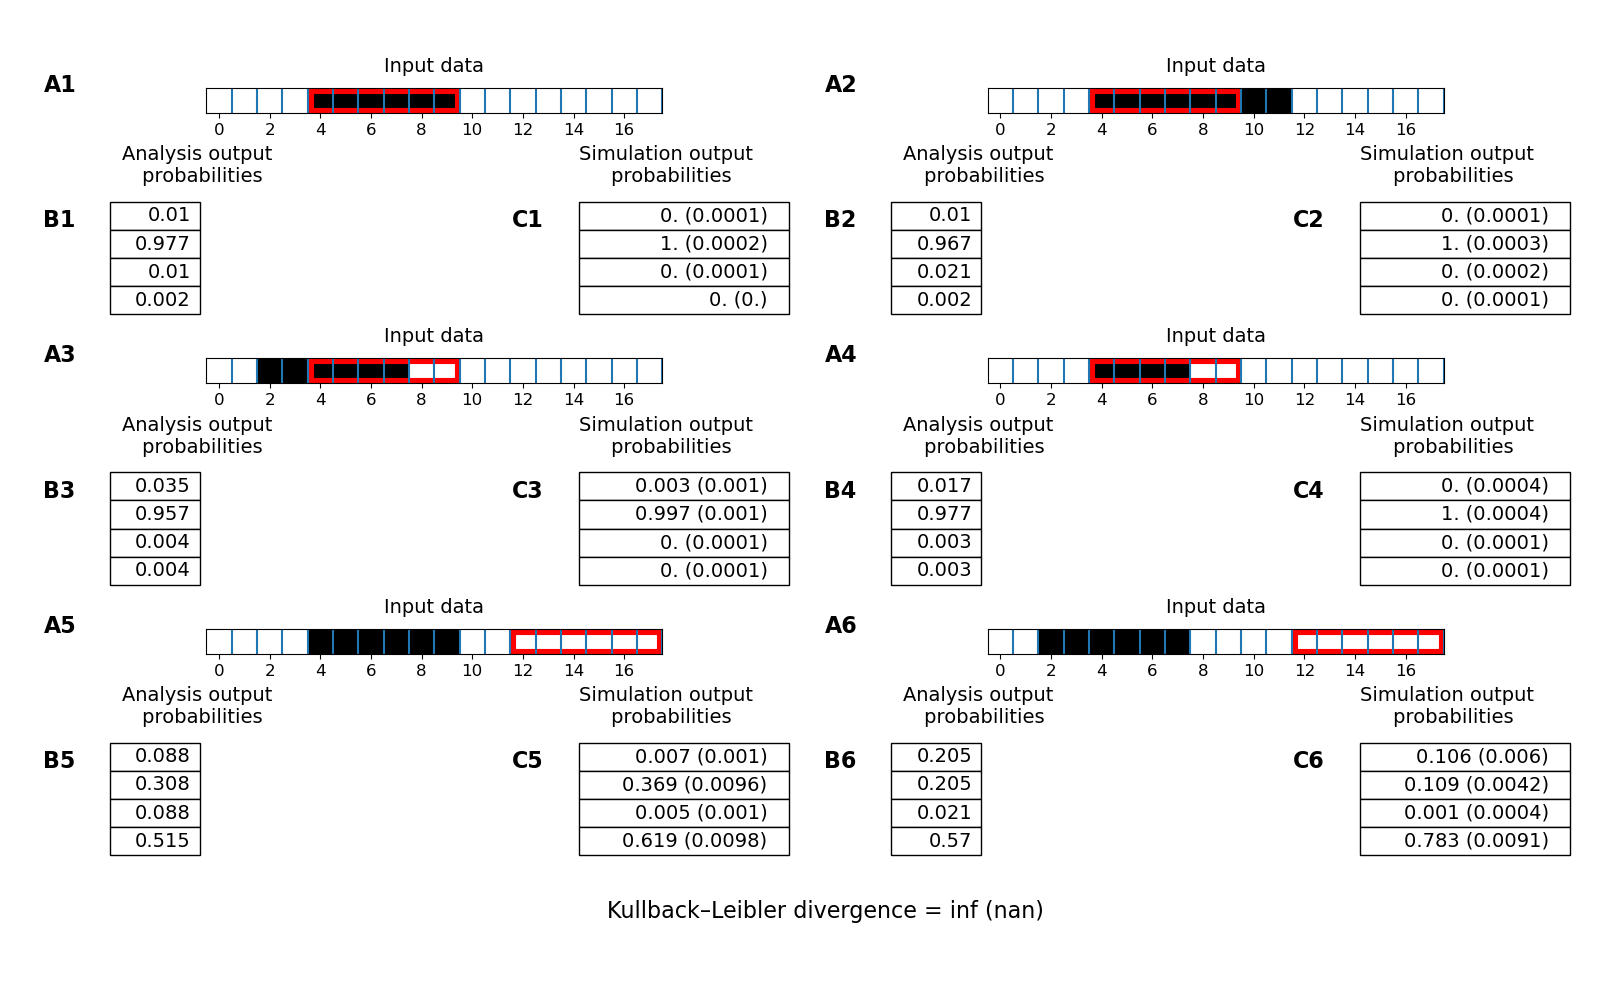
\includegraphics[width=\linewidth]{figures/1D/doubleSize/doubleSize_98_880_4.png}
      \caption{\textbf{Analysis and simulation result. } Hyperparameters: $f_{input} = 98 Hz, f_{prior} = 880 Hz, \tau_{decay} = 4 ms$ \textbf{A} Input images with 18 x 1 pixels. Prior given as red border. \textbf{B} Analytically calculated posterior probabilities and simulated posterior probabilities. The standard deviations are given by the black bars.}
  \label{fig:doubleSize_98_880_4}
\end{figure}

\begin{table}[]
\label{tab:doubleSize_98_880_4}
\small
\tabcolsep=0.11cm
\begin{tabular}{|c|cc|cc|}
\hline
                       & \multicolumn{2}{c|}{Image 1}                       & \multicolumn{2}{c|}{Image 2}                       \\ \hline
                       & \multicolumn{1}{c|}{Analysis} & Simulation         & \multicolumn{1}{c|}{Analysis} & Simulation         \\ \hline
$y_0$                  & \multicolumn{1}{c|}{0.010}    & 0.000 $\pm$ 0.0001 & \multicolumn{1}{c|}{0.010}    & 0.000 $\pm$ 0.0001 \\ \hline
$y_1$                  & \multicolumn{1}{c|}{0.977}    & 1.000 $\pm$ 0.0002 & \multicolumn{1}{c|}{0.967}    & 1.000 $\pm$ 0.0003 \\ \hline
$y_2$                  & \multicolumn{1}{c|}{0.010}    & 0.000 $\pm$ 0.0001 & \multicolumn{1}{c|}{0.021}    & 0.000 $\pm$ 0.0002 \\ \hline
$y_3$                  & \multicolumn{1}{c|}{0.002}    & 0.000 $\pm$ 0.0000 & \multicolumn{1}{c|}{0.002}    & 0.000 $\pm$ 0.0001 \\ \hline
                       & \multicolumn{2}{c|}{Image 3}                       & \multicolumn{2}{c|}{Image 4}                       \\ \hline
$y_0$                  & \multicolumn{1}{c|}{0.035}    & 0.003 $\pm$ 0.0010 & \multicolumn{1}{c|}{0.017}    & 0.000 $\pm$ 0.0004 \\ \hline
$y_1$                  & \multicolumn{1}{c|}{0.957}    & 0.997 $\pm$ 0.0010 & \multicolumn{1}{c|}{0.977}    & 1.000 $\pm$ 0.0004 \\ \hline
$y_2$                  & \multicolumn{1}{c|}{0.004}    & 0.000 $\pm$ 0.0001 & \multicolumn{1}{c|}{0.003}    & 0.000 $\pm$ 0.0001 \\ \hline
$y_3$                  & \multicolumn{1}{c|}{0.004}    & 0.000 $\pm$ 0.0001 & \multicolumn{1}{c|}{0.003}    & 0.000 $\pm$ 0.0001 \\ \hline
						& \multicolumn{2}{c|}{Image 5}                       & \multicolumn{2}{c|}{Image 6}                       \\ \hline
$y_0$                  & \multicolumn{1}{c|}{0.088}    & 0.007 $\pm$ 0.0010 & \multicolumn{1}{c|}{0.205}    & 0.106 $\pm$ 0.0060 \\ \hline
$y_1$                  & \multicolumn{1}{c|}{0.308}    & 0.369 $\pm$ 0.0096 & \multicolumn{1}{c|}{0.205}    & 0.109 $\pm$ 0.0042 \\ \hline
$y_2$                  & \multicolumn{1}{c|}{0.088}    & 0.005 $\pm$ 0.0010 & \multicolumn{1}{c|}{0.021}    & 0.001 $\pm$ 0.0004 \\ \hline
$y_3$                  & \multicolumn{1}{c|}{0.515}    & 0.619 $\pm$ 0.0098 & \multicolumn{1}{c|}{0.570}    & 0.783 $\pm$ 0.0091 \\ \hline
\end{tabular}
\caption{\textbf{Analysis and simulation output probabilities. } Hyperparameters: $f_{input} = 98 Hz, f_{prior} = 880 Hz, \tau_{decay} = 4 ms$}
\end{table}

\section{Experiment 4: Training of the network with 1-D images and predetermined hyperparameters}
\label{section:1DPreDetermined}

\subsection{Introduction}

In this Experiment the network of Experiment 2 was used, but the weights of the network were not derived from the matrices $P^{X|Y}$ and $P^{Y|Z}$, but they were learned from the input images. This was done to analyse how well the optimal weights and the posterior could be approximated with the predetermined hyperparameters.

\subsection{Methods}

The network architecture was the same as in Experiment 2 and the training paradigm was the same as in Experiment 1. The used hyperparameters were $f_{input} = 98 Hz$, $f_{prior} = 440 Hz$ and $\tau_{decay} = 4 ms$. The weight shifting hyperparameter c was determined via grid search.
\subsection{Results}

The Kullback-Leibler divergence for different values of c can be seen in Figure \ref{fig:1DTrainingC}.
\begin{figure}
\centering
  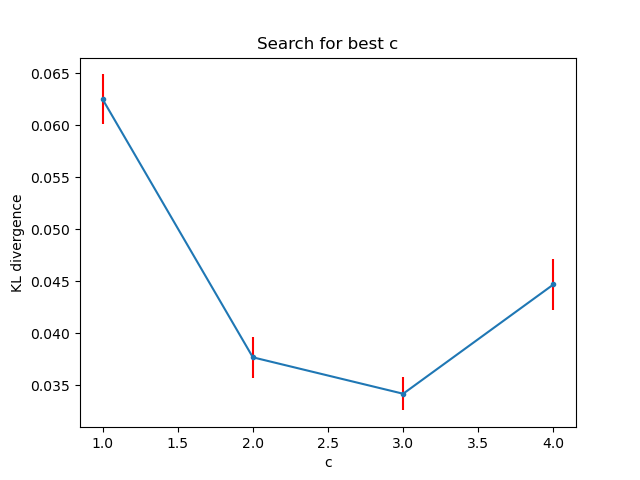
\includegraphics[width=0.75\linewidth]{figures/1D/training/KLD_cvsfInput98_fPrior440tau4.png}
  \caption{\textbf{KL divergence for different c values} $f_{input} = 98 Hz, f_{prior} = 440 Hz, \tau_{decay} = 4 ms$}
  \label{fig:1DTrainingC}
\end{figure}

The training and evaluation results for the best value of $c = 3$ can be seen in Figures \ref{fig:1DTrainingC3}, Figure \ref{fig:1DTrainingEvaluationC3} and Table \ref{tab:1DTrainingEvaluationC3}.
\begin{figure}
  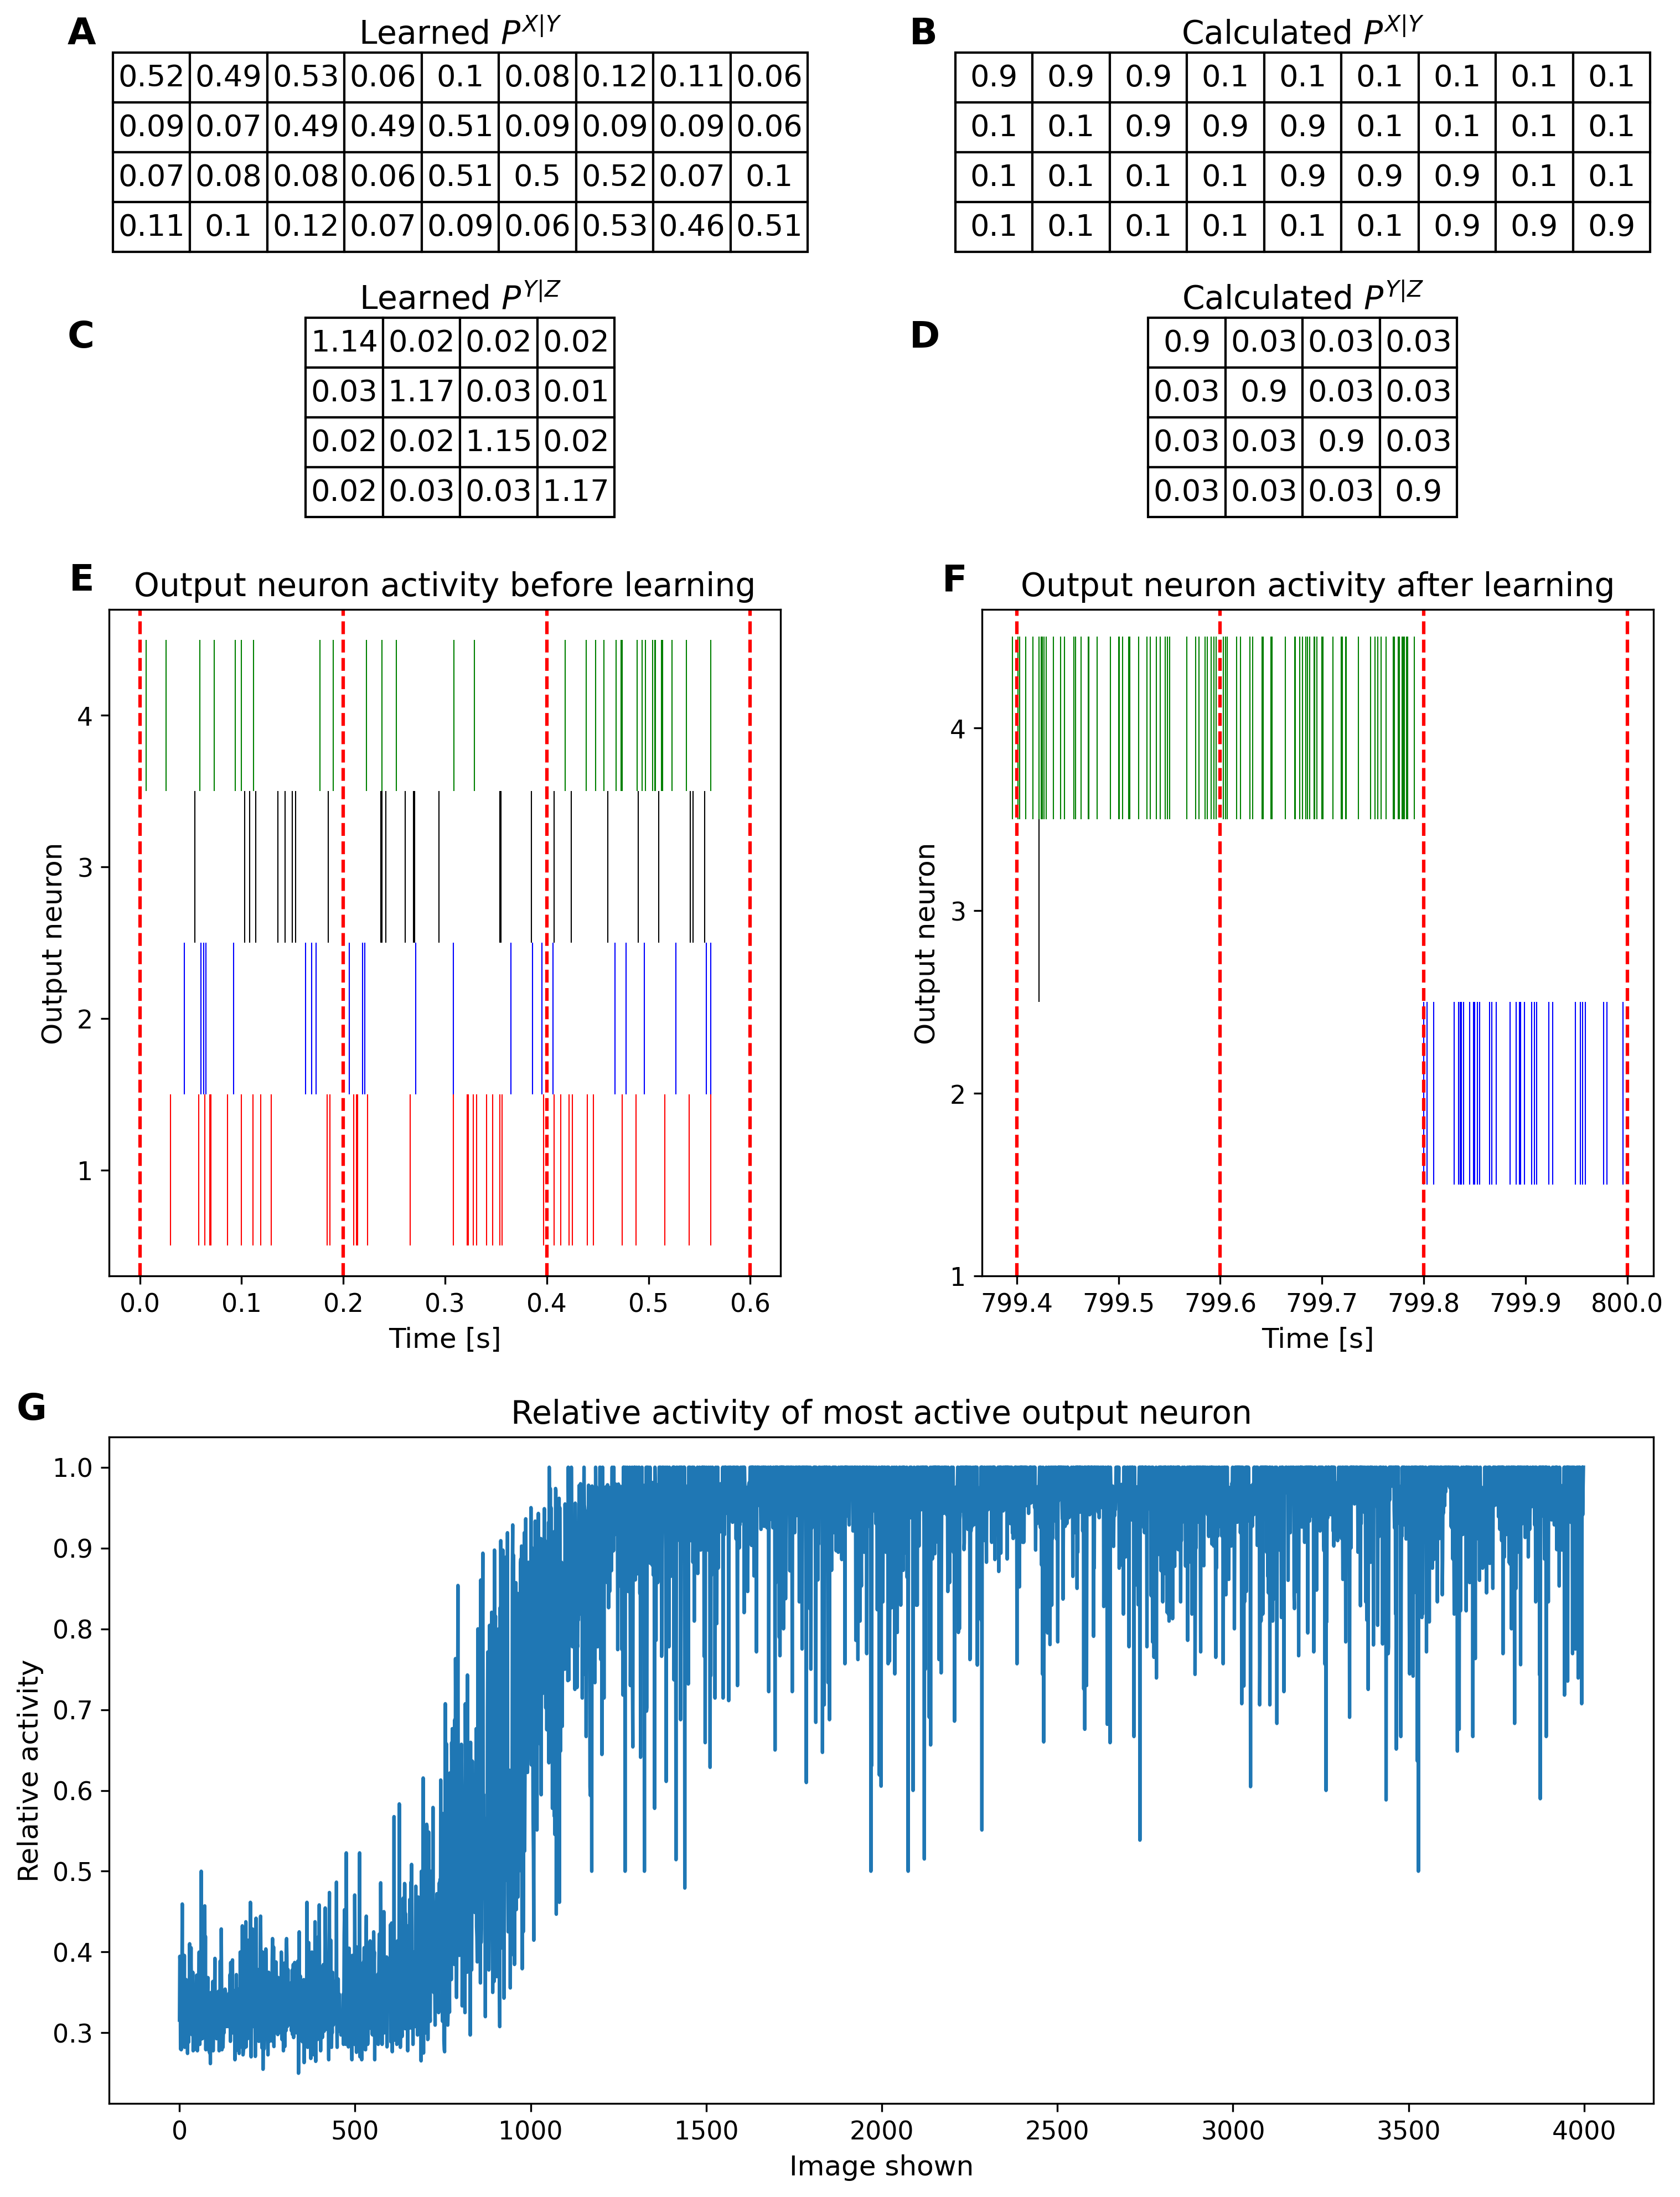
\includegraphics[width=0.8\linewidth]{figures/1D/training/trainingPlot_98_440_4_c3.png}
  \caption{\textbf{Training result.} Hyperparameters: $f_{input} = 98 Hz, f_{prior} = 440 Hz, \tau_{decay} = 4 ms, c = 3$  \textbf{A} The learned probability matrix $P^{X|Y}$. It was determined by taking the weights to the power of e. \textbf{B} The calculated probability matrix $P^{X|Y}$. \textbf{C} The learned prior probability matrix $P^{Y|Z}$. \textbf{D} The calculated prior probability matrix $P^{Y|Z}$.
 \textbf{E, F} Spike activity expressed by the output neurons before and after the training of the network. \textbf{G} This shows the number of spikes the most active output neuron generated, relative to the number of spikes all other output neurons generated combined.}
  \label{fig:1DTrainingC3}
\end{figure}

\begin{figure}
  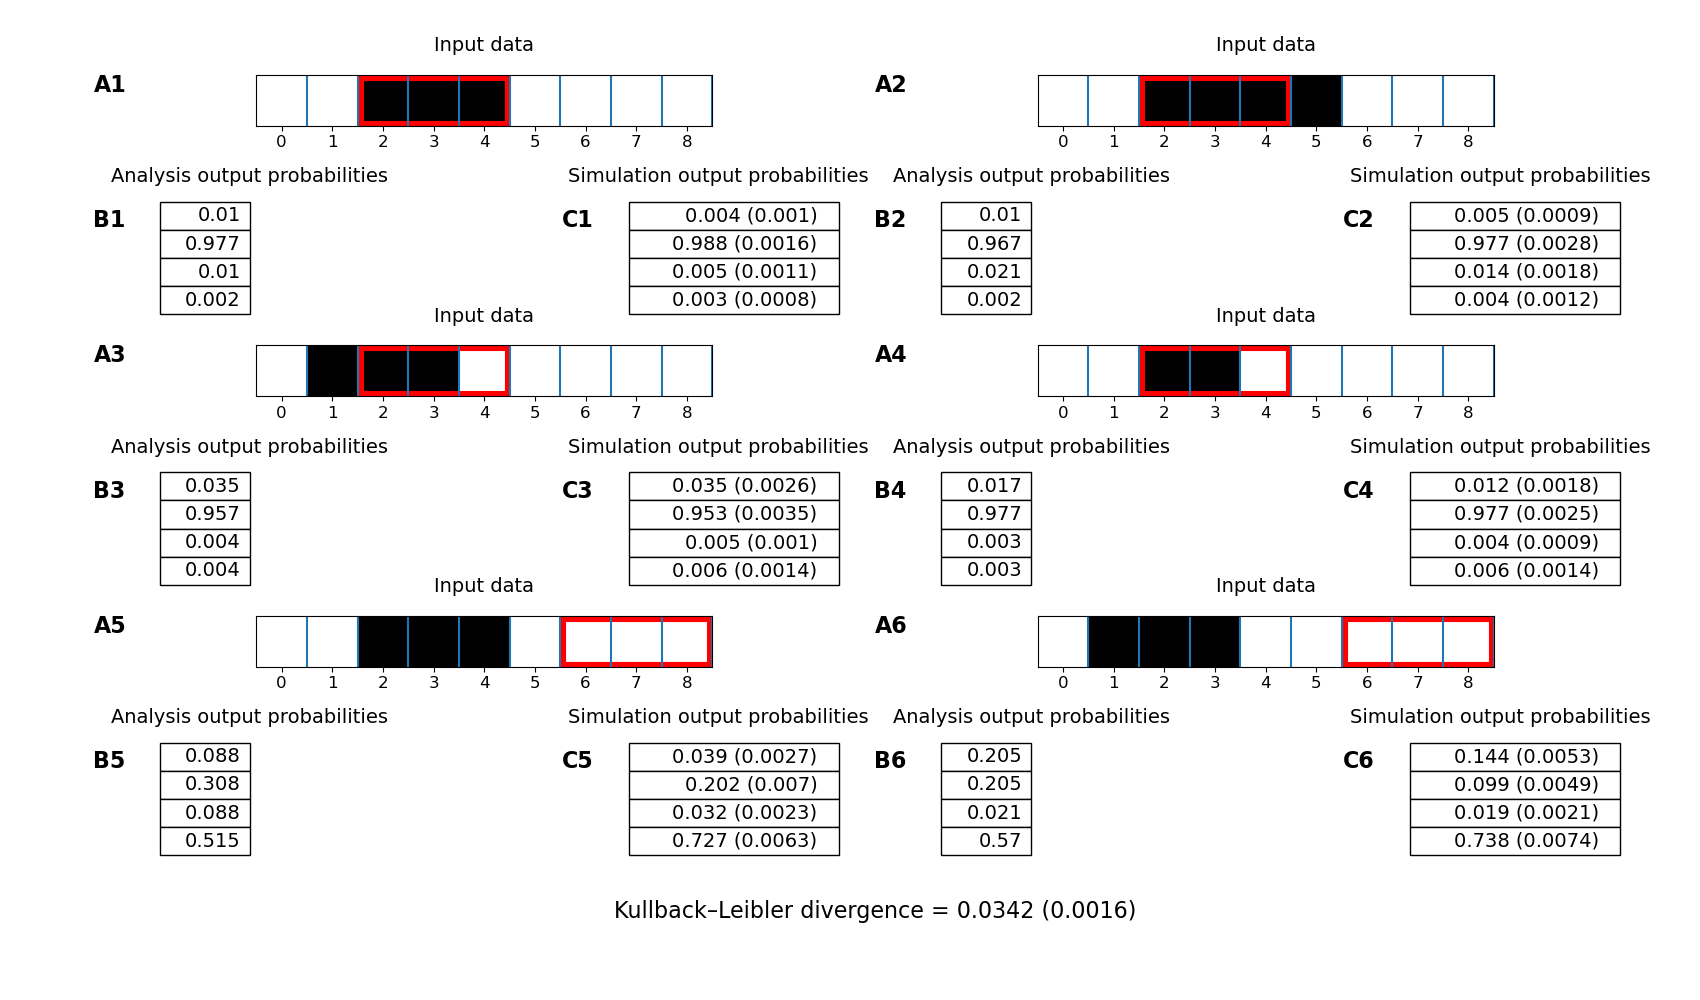
\includegraphics[width=\linewidth]{figures/1D/training/trainingEvaluation_98_440_4_c3.png}
      \caption{\textbf{Analysis and simulation result. } Hyperparameters: $f_{input} = 98 Hz, f_{prior} = 440 Hz, \tau_{decay} = 4 ms, c = 3$ \textbf{A} Input images with 9 x 1 pixels. Prior given as red border. \textbf{B} Analytically calculated posterior probabilities and simulated posterior probabilities. The standard deviations are given by the black bars.}  
  \label{fig:1DTrainingEvaluationC3}
\end{figure}

\begin{table}[]
\label{tab:1DTrainingEvaluationC3}
\small
\tabcolsep=0.11cm
\begin{tabular}{|c|cc|cc|}
\hline
                       & \multicolumn{2}{c|}{Image 1}                       & \multicolumn{2}{c|}{Image 2}                       \\ \hline
                       & \multicolumn{1}{c|}{Analysis} & Simulation         & \multicolumn{1}{c|}{Analysis} & Simulation         \\ \hline
$y_0$                  & \multicolumn{1}{c|}{0.010}    & 0.004 $\pm$ 0.0010 & \multicolumn{1}{c|}{0.010}    & 0.005 $\pm$ 0.0009 \\ \hline
$y_1$                  & \multicolumn{1}{c|}{0.977}    & 0.988 $\pm$ 0.0016 & \multicolumn{1}{c|}{0.967}    & 0.977 $\pm$ 0.0028 \\ \hline
$y_2$                  & \multicolumn{1}{c|}{0.010}    & 0.005 $\pm$ 0.0011 & \multicolumn{1}{c|}{0.021}    & 0.014 $\pm$ 0.0.0018 \\ \hline
$y_3$                  & \multicolumn{1}{c|}{0.002}    & 0.003 $\pm$ 0.0008 & \multicolumn{1}{c|}{0.002}    & 0.004 $\pm$ 0.0012 \\ \hline
                       & \multicolumn{2}{c|}{Image 3}                       & \multicolumn{2}{c|}{Image 4}                       \\ \hline
$y_0$                  & \multicolumn{1}{c|}{0.035}    & 0.035 $\pm$ 0.0026 & \multicolumn{1}{c|}{0.017}    & 0.012 $\pm$ 0.0018 \\ \hline
$y_1$                  & \multicolumn{1}{c|}{0.957}    & 0.953 $\pm$ 0.0035 & \multicolumn{1}{c|}{0.977}    & 0.977 $\pm$ 0.0025 \\ \hline
$y_2$                  & \multicolumn{1}{c|}{0.004}    & 0.005 $\pm$ 0.0010 & \multicolumn{1}{c|}{0.003}    & 0.004 $\pm$ 0.0009 \\ \hline
$y_3$                  & \multicolumn{1}{c|}{0.004}    & 0.006 $\pm$ 0.0014 & \multicolumn{1}{c|}{0.003}    & 0.006 $\pm$ 0.0014 \\ \hline
						& \multicolumn{2}{c|}{Image 5}                       & \multicolumn{2}{c|}{Image 6}                       \\ \hline
$y_0$                  & \multicolumn{1}{c|}{0.088}    & 0.039 $\pm$ 0.0027 & \multicolumn{1}{c|}{0.205}    & 0.144 $\pm$ 0.0053 \\ \hline
$y_1$                  & \multicolumn{1}{c|}{0.308}    & 0.202 $\pm$ 0.0070 & \multicolumn{1}{c|}{0.205}    & 0.099 $\pm$ 0.0049 \\ \hline
$y_2$                  & \multicolumn{1}{c|}{0.088}    & 0.032 $\pm$ 0.0023 & \multicolumn{1}{c|}{0.021}    & 0.019 $\pm$ 0.0021 \\ \hline
$y_3$                  & \multicolumn{1}{c|}{0.515}    & 0.727 $\pm$ 0.0063 & \multicolumn{1}{c|}{0.570}    & 0.738 $\pm$ 0.0074 \\ \hline
\end{tabular}
\caption{\textbf{Analysis and simulation output probabilities. } Hyperparameters: $f_{input} = 98 Hz, f_{prior} = 440 Hz, \tau_{decay} = 4 ms, c = 3$}
\end{table}